\chapter{Diseño de la solución}\label{cap:diseño}

\section{Introducción}

En este capítulo se describe el diseño de la solución adoptada para el sistema \textbf{Sevillaneando}. El diseño parte de los requisitos identificados en el capítulo anterior y define la arquitectura general del sistema, el modelo de datos, la interfaz de usuario y el flujo de navegación de la aplicación.

El objetivo de este capítulo es explicar las decisiones estructurales tomadas antes y durante la implementación, justificando por qué se han elegido determinados patrones y organizaciones frente a otras alternativas posibles.

\section{Arquitectura del sistema}

El sistema \textbf{Sevillaneando} sigue una arquitectura cliente-servidor distribuida en dos capas principales: una aplicación móvil que actúa como cliente y un servidor backend que expone una API REST. Además, el sistema se apoya en servicios externos para cubrir necesidades específicas como autenticación, almacenamiento de imágenes y obtención de datos de fuentes externas.

La figura~\ref{fig:vista_logica} muestra la vista lógica del sistema con los componentes principales y sus relaciones.

\begin{figure}[H]
    \centering
    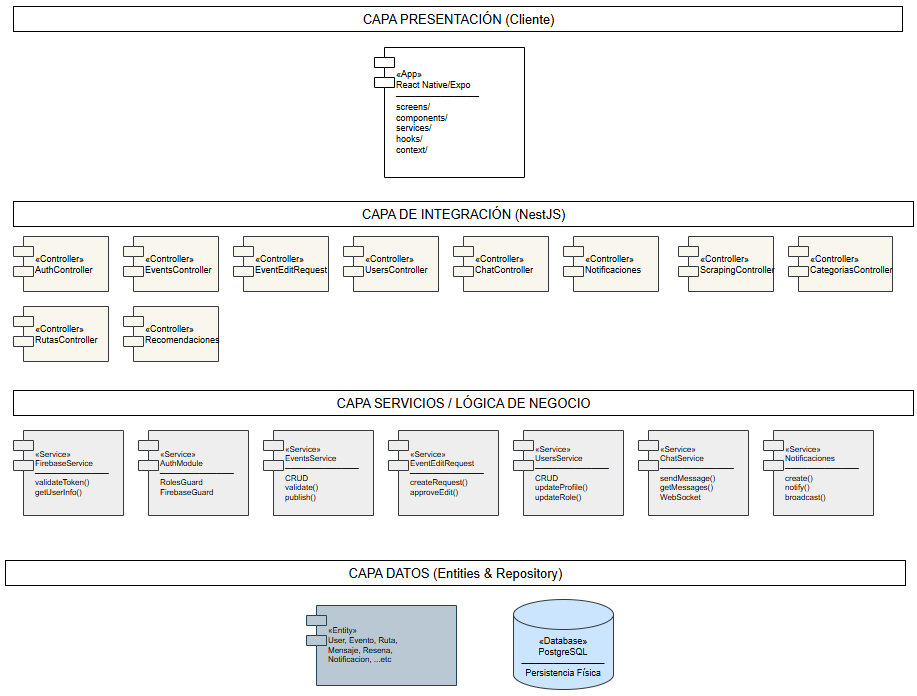
\includegraphics[width=\textwidth]{figures/vistas/vista_logica.png}
    \caption{Vista lógica del sistema Sevillaneando}
    \label{fig:vista_logica}
\end{figure}

\subsection{Aplicación móvil (frontend)}

La aplicación móvil actúa como único punto de interacción con el usuario. Ha sido desarrollada con \textbf{React Native}~\cite{reactnative} y \textbf{Expo}~\cite{expo}, lo que permite generar una única base de código compatible con Android e iOS. La versión final del cliente contiene 83 ficheros TypeScript/TSX en \texttt{src}, con 17.774 líneas de código distribuidas en pantallas, componentes, navegación, servicios, contextos, hooks, tipos y utilidades. La arquitectura interna del frontend se estructura en los siguientes niveles:

\begin{itemize}
    \item \textbf{Pantallas}: 31 componentes que representan vistas completas navegables.
    \item \textbf{Componentes}: 11 elementos reutilizables que componen la interfaz, como botones temáticos, cabeceras de perfil, selectores, esqueletos de carga, modales y atribuciones de OpenStreetMap.
    \item \textbf{Servicios}: capa de comunicación con el backend mediante \textbf{Axios}. Todos los servicios comparten un cliente Axios centralizado que inyecta automáticamente el token de Firebase en la cabecera \texttt{Authorization} de cada petición, gestiona un \textit{timeout} global de 60 segundos y aplica un interceptor de reintento ante errores de red.
    \item \textbf{Contextos}: gestión del estado global compartido entre pantallas (\texttt{AuthContext} para la sesión, \texttt{SocketContext} para la conexión WebSocket, \texttt{ThemeContext} para el tema visual y \texttt{NotificacionesContext} para los avisos pendientes).
\end{itemize}

La navegación entre pantallas se implementa con \textbf{React Navigation}~\cite{reactnavigation} mediante una navegación en pila (\textit{stack navigator}), separando las rutas autenticadas de las públicas. El \texttt{AuthContext} determina en tiempo de montaje qué pila de navegación se activa según el estado de la sesión.

La figura~\ref{fig:flujo_frontend} muestra cómo interactúan estos niveles desde la acción del usuario hasta la respuesta del servidor.

\begin{figure}[H]
\centering
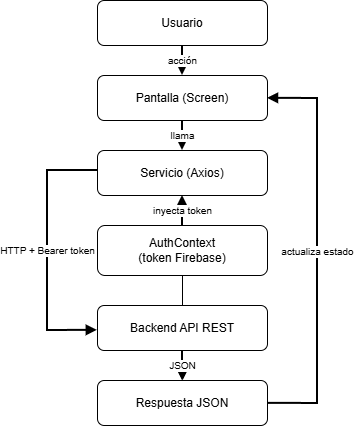
\includegraphics[width=0.65\textwidth]{figures/flujo_frontend.png}
\caption{Flujo de una petición en el frontend desde la acción del usuario hasta la actualización de la pantalla}
\label{fig:flujo_frontend}
\end{figure}

\subsection{Servidor backend}

El backend es una API REST desarrollada con \textbf{NestJS}~\cite{nestjs} sobre \textbf{Node.js}. NestJS organiza el servidor en módulos independientes, cada uno con sus controladores, servicios y entidades. Esta separación facilita el mantenimiento y permite extender el sistema sin afectar al resto de componentes.

Cada petición HTTP entrante pasa por la siguiente cadena de responsabilidades:

\begin{enumerate}
    \item \textbf{Guards}: \texttt{FirebaseAuthGuard} intercepta la petición, extrae el token \texttt{Bearer} de la cabecera \texttt{Authorization} y lo verifica con el SDK de administración de Firebase. Si el token es inválido o ha expirado, la petición es rechazada con \texttt{401 Unauthorized} antes de llegar al controlador.
    \item \textbf{Controlador}: recibe la petición validada, extrae los parámetros de ruta, \textit{query} y cuerpo, y delega la lógica de negocio en el servicio correspondiente.
    \item \textbf{Servicio}: ejecuta la lógica de negocio, interactúa con TypeORM para consultar o modificar la base de datos, y si es necesario llama a servicios externos (por ejemplo, Cloudinary para imágenes).
    \item \textbf{TypeORM}: traduce las operaciones del servicio en consultas SQL optimizadas y gestiona la conexión con PostgreSQL.
\end{enumerate}

La figura~\ref{fig:flujo_backend} ilustra esta cadena para una petición autenticada típica.

\begin{figure}[H]
\centering
\begin{tikzpicture}[
    node distance=0.5cm and 2.2cm,
    every node/.style={font=\small},
    box/.style={draw, rounded corners=3pt, minimum width=3.2cm, minimum height=0.7cm, align=center, fill=white},
    ext/.style={draw, rounded corners=3pt, minimum width=2.8cm, minimum height=0.7cm, align=center, fill=gray!12},
    arr/.style={-{Stealth[length=5pt]}, thick},
]
\node[box] (req)   {Petición HTTP};
\node[box, below=of req]   (guard)  {FirebaseAuthGuard};
\node[box, below=of guard] (ctrl)   {Controller};
\node[box, below=of ctrl]  (svc)    {Service};
\node[box, below=of svc]   (orm)    {TypeORM};
\node[box, below=of orm]   (db)     {PostgreSQL + PostGIS};

\node[ext, right=2.6cm of guard] (fbadmin) {Firebase Admin SDK};
\node[ext, right=2.6cm of svc]   (cld)     {Cloudinary};

\draw[arr] (req)   -- (guard);
\draw[arr] (guard) -- node[right, font=\tiny] {token OK} (ctrl);
\draw[arr] (ctrl)  -- (svc);
\draw[arr] (svc)   -- (orm);
\draw[arr] (orm)   -- (db);

\draw[arr] (guard) -- node[above, font=\tiny] {verifica} (fbadmin);
\draw[arr] (svc)   -- node[above, font=\tiny] {upload/delete} (cld);
\end{tikzpicture}
\caption{Cadena de responsabilidades en el backend para una petición autenticada}
\label{fig:flujo_backend}
\end{figure}

La figura~\ref{fig:flujo_autenticacion} muestra en detalle el flujo completo de autenticación, desde el inicio de sesión del usuario hasta la verificación del token en el backend.

\begin{figure}[H]
\centering
\begin{tikzpicture}[
    node distance=1.0cm and 2.4cm,
    every node/.style={font=\small},
    box/.style={draw, rounded corners=3pt, minimum width=3.0cm, minimum height=0.72cm, align=center, fill=white},
    ext/.style={draw, rounded corners=3pt, minimum width=3.0cm, minimum height=0.72cm, align=center, fill=gray!12},
    arr/.style={-{Stealth[length=5pt]}, thick},
]
% Columna izquierda
\node[box] (app)    {App móvil};
\node[box, below=of app]   (sdk)   {Firebase SDK (cliente)};
\node[box, below=of sdk]   (axios) {Axios (interceptor)};
\node[box, below=of axios] (be)    {Backend NestJS};
\node[box, below=of be]    (guard) {FirebaseAuthGuard};

% Columna derecha
\node[ext, right=3.2cm of sdk]   (fbauth) {Firebase Authentication};
\node[ext, right=3.2cm of guard] (fbadm)  {Firebase Admin SDK};

% Flechas
\draw[arr] (app)    -- node[right, font=\tiny] {email + pass} (sdk);
\draw[arr] (sdk)    to[bend left=15]  node[above, font=\tiny] {signIn()} (fbauth);
\draw[arr] (fbauth) to[bend left=15]  node[below, font=\tiny] {JWT (60 min)} (sdk);
\draw[arr] (sdk)    -- node[right, font=\tiny] {token} (axios);
\draw[arr] (axios)  -- node[right, font=\tiny] {Authorization: Bearer \{token\}} (be);
\draw[arr] (be)     -- (guard);
\draw[arr] (guard)  to[bend left=15]  node[above, font=\tiny] {verifyIdToken()} (fbadm);
\draw[arr] (fbadm)  to[bend left=15]  node[below, font=\tiny] {uid + claims} (guard);
\end{tikzpicture}
\caption{Flujo de autenticación: desde el inicio de sesión hasta la verificación del token en el backend}
\label{fig:flujo_autenticacion}
\end{figure}

Además de la API REST, el backend integra un servidor \textbf{Socket.IO}~\cite{socketio} para la comunicación en tiempo real del chat. La conexión WebSocket se autentica en el \textit{handshake} inicial mediante el mismo mecanismo que la API REST: el cliente envía el token de Firebase como parámetro de la URL de conexión, y el middleware de Socket.IO lo verifica antes de aceptar la conexión. Una vez autenticada, la conexión se mantiene abierta y el servidor puede emitir eventos al cliente en cualquier momento sin necesidad de una nueva petición.

\subsection{Base de datos}

La persistencia de datos se gestiona con \textbf{PostgreSQL 15} junto con la extensión \textbf{PostGIS}~\cite{postgisdocs}. PostgreSQL cubre el modelo relacional general del sistema, mientras que PostGIS añade soporte para datos geográficos, permitiendo almacenar coordenadas como puntos \texttt{geography} en SRID 4326 y ejecutar consultas espaciales eficientes como el filtrado por radio (\texttt{ST\_DWithin}) o el cálculo de distancias en metros (\texttt{ST\_Distance}). La comunicación entre el backend y la base de datos se realiza a través de \textbf{TypeORM}~\cite{typeorm}, que mapea las entidades TypeScript a tablas SQL y genera las consultas correspondientes.

\subsection{Servicios externos}

El sistema delega en servicios externos las siguientes responsabilidades:

\begin{itemize}
    \item \textbf{Firebase Authentication}~\cite{firebase}: gestión del ciclo de vida de la sesión del usuario (registro, inicio de sesión y tokens JWT). El cliente móvil usa el SDK de Firebase para obtener y renovar tokens; el backend usa el SDK de administración para verificarlos sin almacenar contraseñas ni gestionar sesiones propias.
    \item \textbf{Cloudinary}~\cite{cloudinary}: almacenamiento y servicio de imágenes asociadas a eventos, perfiles y chats. El backend sube las imágenes directamente a Cloudinary mediante su SDK y almacena únicamente la URL resultante en PostgreSQL. Cloudinary sirve las imágenes desde su CDN (Content Delivery Network) con transformaciones automáticas de formato y calidad.
    \item \textbf{OpenStreetMap}~\cite{openstreetmap}: visualización de mapas interactivos en el frontend mediante \texttt{react-native-maps}. Los \textit{tiles} cartográficos se obtienen directamente del servidor de OpenStreetMap sin pasar por el backend.
    \item \textbf{Eventbrite}~\cite{eventbrite} \textbf{/ Ticketmaster}~\cite{ticketmaster} \textbf{/ Visita Sevilla / webs institucionales y de ocio de Sevilla}: fuentes externas de eventos consultadas automáticamente mediante scraping. Eventbrite se procesa extrayendo tarjetas de eventos y bloques JSON-LD del HTML; la API oficial de Ticketmaster se consume directamente; el portal \texttt{visitasevilla.es} dispone de un scraper dedicado que interpreta su formato de fechas propio; el resto de webs (portal municipal, guías de ocio, teatros y fundaciones) se procesan mediante el \texttt{GeminiScraperService}, que envía el texto limpio de cada página al modelo \textbf{Gemini 2.5 Flash} (Google Generative AI) y obtiene los eventos en formato JSON estructurado. El backend ejecuta diariamente un \textit{cron job} que invoca cada scraper, transforma los datos al modelo interno y los persiste en PostgreSQL asignándolos al usuario técnico \textit{scraper-bot}.
\end{itemize}

\begin{itemize}
    \item \textbf{Nominatim (OpenStreetMap)}: API de geocodificación utilizada por el \texttt{GeminiScraperService} para resolver las coordenadas geográficas de los eventos cuando Gemini no puede deducirlas directamente del texto. Se realizan hasta tres variantes de búsqueda por dirección para maximizar la cobertura.
\end{itemize}

La figura~\ref{fig:conexion_tecnologias} resume cómo se conectan todas las tecnologías del sistema en tiempo de ejecución, mostrando el camino que recorre una petición desde que el usuario interactúa con la aplicación hasta que los datos son persistidos o devueltos.

\begin{figure}[H]
\centering
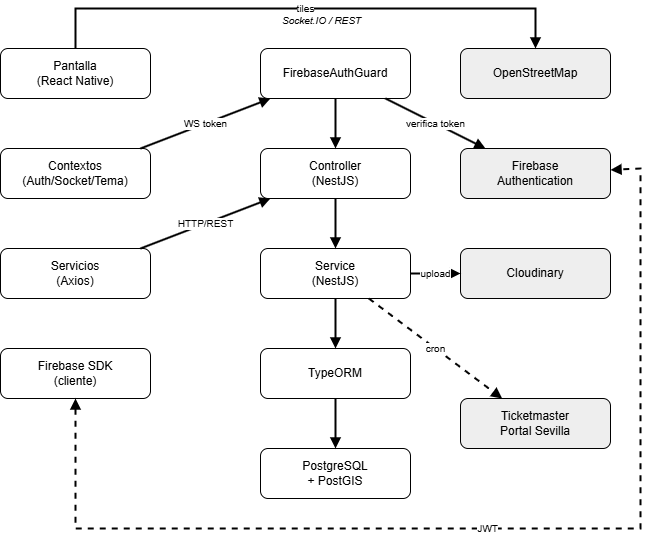
\includegraphics[width=0.95\textwidth]{figures/conexion_tecnologias.png}
\caption{Conexión entre tecnologías del sistema en tiempo de ejecución}
\label{fig:conexion_tecnologias}
\end{figure}

Una vez descritos los componentes internos y los servicios externos, la figura~\ref{fig:vista_despliegue} sitúa esos elementos sobre la infraestructura de ejecución utilizada por el sistema.

\begin{figure}[H]
\centering
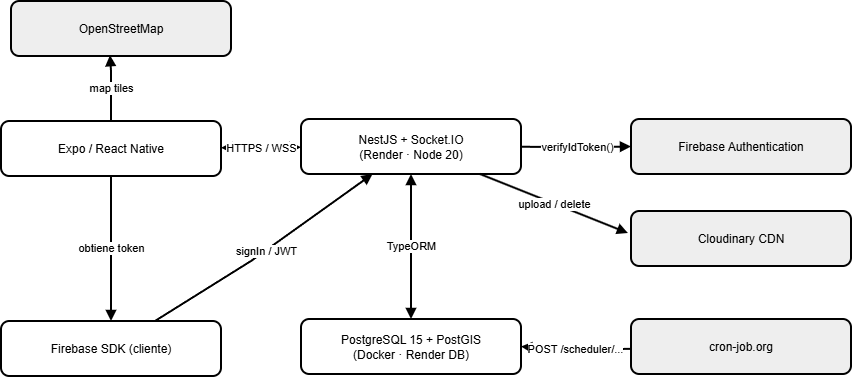
\includegraphics[width=0.95\textwidth]{figures/vistas/vista_despliegue.png}
\caption{Vista de despliegue del sistema Sevillaneando}
\label{fig:vista_despliegue}
\end{figure}

\section{Modelo de datos}

El modelo de datos del sistema refleja las entidades identificadas en el análisis y las relaciones entre ellas. La tabla~\ref{tab:entidades} describe las entidades principales y sus atributos más relevantes.

{\renewcommand{\arraystretch}{1.25}
\begin{longtable}{@{}>{\raggedright\arraybackslash}p{0.22\textwidth} >{\raggedright\arraybackslash}p{0.72\textwidth}@{}}
\caption{Entidades del modelo de datos}
\label{tab:entidades}\\
\toprule
\textbf{Entidad} & \textbf{Descripción y atributos principales} \\
\midrule
\endfirsthead
\toprule
\textbf{Entidad} & \textbf{Descripción y atributos principales} \\
\midrule
\endhead
\bottomrule
\endfoot
\texttt{User} & Representa a cada persona registrada. Atributos: UUID, UID de Firebase, correo, nombre, foto de perfil (\texttt{fotoPerfilPublicId} en Cloudinary), ubicación geográfica (punto PostGIS SRID 4326), rol (\texttt{user}, \texttt{moderator} o \texttt{admin}), intereses por categoría, fecha de aceptación de privacidad (\texttt{privacyAcceptedAt}), orden de categorías personalizado (\texttt{categoryOrder}) y radios de búsqueda configurados (\texttt{radiusOptions}). \\
\addlinespace
\texttt{Event} & Representa un evento cultural o de ocio. Atributos: título, descripción, dirección, ubicación geográfica (punto PostGIS SRID 4326), fechas de inicio y fin, precio fijo o en rango, imagen principal, hasta cinco imágenes adicionales, estado de moderación (\texttt{Pendiente}, \texttt{Aprobado} o \texttt{Rechazado}), visibilidad, enlace de acceso para eventos privados (\texttt{linkAcceso}), recurrencia (\texttt{diario}, \texttt{semanal}, \texttt{quincenal} o \texttt{mensual}), fecha final de recurrencia e indicador \texttt{hasMultipleDatesAvailable} para eventos con varias sesiones. \\
\addlinespace
\texttt{Categoria} & Clasifica los eventos por temática. Contiene nombre y descripción. Solo los administradores pueden crearlas, editarlas o eliminarlas. \\
\addlinespace
\texttt{Resena} & Valoración de un evento por parte de un usuario. Incluye puntuación de 1 a 5 estrellas, comentario opcional, referencia al usuario autor y al evento valorado. \\
\addlinespace
\texttt{Mensaje} & Mensaje del chat grupal de un evento. Incluye contenido de texto, URL de imagen opcional, usuario emisor y referencia al evento. \\
\addlinespace
\texttt{MensajePrivado} & Mensaje directo entre dos usuarios. Contiene contenido, imagen opcional, referencias a emisor y receptor, e indicador de lectura (\texttt{leido}). \\
\addlinespace
\texttt{Notificacion} & Aviso enviado a un usuario. Incluye tipo (aprobación, rechazo, evento cercano, evento próximo, mensaje privado, nuevo seguidor o recomendación), mensaje, estado de lectura, y referencias auxiliares opcionales al evento relacionado (\texttt{targetEventId}) o al usuario origen (\texttt{sourceUserId}) para navegar directamente a la pantalla correspondiente. \\
\addlinespace
\texttt{Ruta} & Itinerario formado por una secuencia ordenada de eventos. Almacena título, descripción, secuencia de eventos (M:N con \texttt{Event}), trayecto geográfico (array de puntos GeoJSON), duración estimada en minutos, creador, puntuación promedio y número de calificaciones recibidas. \\
\addlinespace
\texttt{CalificacionRuta} & Valoración de un usuario sobre una ruta. Almacena puntuación numérica y fechas de creación y actualización. Restricción de unicidad compuesta (usuario, ruta): cada usuario solo puede calificar una ruta una vez. Se borra en cascada al eliminar el usuario o la ruta. \\
\addlinespace
\texttt{Recomendacion} & Sugerencia personalizada generada por el motor de recomendaciones. Almacena los eventos recomendados y los criterios aplicados \\
\addlinespace
\texttt{EventEditRequest} & Solicitud de edición de un evento público creada por su autor. Almacena únicamente los campos que se quieren modificar, todos opcionales: título, descripción, dirección, ubicación, fechas, precio, visibilidad, enlace de acceso e imágenes. El estado se crea siempre como \texttt{pendiente} y solo el moderador puede cambiarlo a \texttt{aprobada} o \texttt{rechazada}. Si se rechaza, puede almacenarse un motivo opcional. Permite separar el contenido publicado de los cambios pendientes de moderación. \\
\end{longtable}
}

El moderador puede además editar directamente los eventos públicos pendientes antes de aprobarlos o rechazarlos, y supervisar cualquier evento público aprobado desde un listado específico. Esta operación no aplica a eventos privados ajenos, que quedan bajo control exclusivo de su creador.

\subsection{Diagrama entidad-relación}

La figura~\ref{fig:edt_modelo} muestra el diagrama entidad-relación del sistema con las relaciones principales entre entidades.

\begin{figure}[H]
    \centering
    
\includegraphics[width=0.95\textwidth]{figures/vistas/vista_de_datos.png}
    \caption{Diagrama entidad-relación del sistema}
    \label{fig:edt_modelo}
\end{figure}

Las relaciones principales entre entidades son las siguientes:

\begin{itemize}
    \item Un usuario puede crear múltiples eventos (1:N) y múltiples rutas (1:N).
    \item Un usuario mantiene cuatro relaciones M:N independientes con los eventos: asistencia (\texttt{event\_asistentes}), guardado (\texttt{user\_saved\_events}), compartición (\texttt{user\_shared\_events}) y visita (\texttt{user\_visited\_events}).
    \item Un usuario puede seguir a otros usuarios mediante una relación reflexiva M:N (\texttt{user\_seguidores}).
    \item Un evento pertenece a una categoría (N:1).
    \item Un evento puede tener múltiples reseñas (1:N) y múltiples mensajes de chat grupal (1:N).
    \item Dos usuarios cualesquiera pueden intercambiar mensajes privados: cada \texttt{MensajePrivado} referencia a un emisor y a un receptor (N:1 hacia \texttt{User} en ambos extremos).
    \item Una notificación pertenece a un único usuario (N:1).
    \item Una ruta contiene una secuencia ordenada de eventos (M:N mediante \texttt{ruta\_eventos}) y puede recibir múltiples calificaciones de usuarios (1:N a \texttt{CalificacionRuta}); cada calificación referencia también al usuario autor (N:1).
    \item Una recomendación pertenece a un usuario (N:1) y agrupa múltiples eventos recomendados para ese usuario (M:N).
\end{itemize}

\section{Diseño de la API REST}

El backend expone una API REST~\cite{fielding2000rest} cuya organización sigue la estructura modular de NestJS. Cada módulo define un conjunto de endpoints agrupados por recurso. La documentación interactiva completa se genera automáticamente mediante \texttt{@nestjs/swagger} y queda disponible en \texttt{/api/docs} cuando el servidor está en ejecución.

\subsection{Versionado}

La API no aplica versionado explícito en la URL (p.ej.\ \texttt{/v1/}) en esta primera versión, dado que cliente y servidor se desarrollan y despliegan de forma coordinada en el mismo proyecto. Si en el futuro el sistema expusiera la API a clientes externos independientes, se adoptaría versionado mediante prefijo de ruta (\texttt{/v1/}, \texttt{/v2/}) o cabecera \texttt{Accept-Version}, siguiendo la convención habitual de NestJS.

\subsection{Autenticación y control de acceso}

Todos los endpoints protegidos reciben el token de Firebase en la cabecera \texttt{Authorization: Bearer <token>}. Los endpoints que exigen un rol específico aplican un guard adicional de roles. En la tabla~\ref{tab:api} la columna \textbf{Auth} indica el acceso funcional expuesto por la aplicación: \textbf{—} (público), \textbf{U} (usuario), \textbf{T} (cualquier rol autenticado: usuario, moderador o administrador), \textbf{C} (creador o propietario del recurso), \textbf{C/M} (creador o moderador sobre evento público), \textbf{M} (solo moderador) o \textbf{A} (solo administrador).

\subsection{Endpoints principales}

La tabla~\ref{tab:api} recoge los endpoints de cada módulo extraídos directamente del contrato OpenAPI exportado desde el backend. El contenido fue generado con asistencia de Claude (Anthropic) a partir del YAML del Swagger y revisado por la autora.

{\scriptsize
\renewcommand{\arraystretch}{1.15}
\newcommand{\apiendpoint}[2]{\begingroup\Urlmuskip=0mu plus 2mu\relax\texttt{#1}\space\path{#2}\endgroup}
\begin{longtable}{|>{\raggedright\arraybackslash}p{1.25cm}|>{\raggedright\arraybackslash}p{3.55cm}|>{\centering\arraybackslash}p{0.75cm}|>{\raggedright\arraybackslash}p{4.0cm}|>{\raggedright\arraybackslash}p{1.8cm}|}
\caption{Endpoints de la API REST (fuente: OpenAPI 3.0)}\label{tab:api}\\
\hline
\textbf{Módulo} & \textbf{Método / Ruta} & \textbf{Auth} & \textbf{Parámetros / Cuerpo} & \textbf{Respuestas} \\
\hline
\endfirsthead
\hline
\textbf{Módulo} & \textbf{Método / Ruta} & \textbf{Auth} & \textbf{Parámetros / Cuerpo} & \textbf{Respuestas} \\
\hline
\endhead
\hline
\endlastfoot

\multirow{19}{=}{Eventos}
 & \apiendpoint{POST}{/events} & U & Body: \texttt{CreateEventDto} & 201, 400, 401 \\
\cline{2-5}
 & \apiendpoint{GET}{/events} & — & Query: \texttt{userId?}, \texttt{lat?}, \texttt{lng?}, \texttt{radiusKm?}, \texttt{limit?}, \texttt{offset?} & 200 \\
\cline{2-5}
 & \apiendpoint{GET}{/events/\{id\}} & — & Path: \texttt{id} (UUID) & 200, 404 \\
\cline{2-5}
 & \apiendpoint{PUT}{/events/\{id\}} & C/M & Path: \texttt{id}; Body: \texttt{UpdateEventDto} & 200, 400, 401, 404 \\
\cline{2-5}
 & \apiendpoint{DELETE}{/events/\{id\}} & C/M & Path: \texttt{id} & 200, 401, 403, 404 \\
\cline{2-5}
 & \apiendpoint{PATCH}{/events/\{id\}/aprobar} & M & Path: \texttt{id} & 200, 401, 403, 404 \\
\cline{2-5}
 & \apiendpoint{PATCH}{/events/\{id\}/rechazar} & M & Path: \texttt{id} & 200, 401, 403, 404 \\
\cline{2-5}
 & \apiendpoint{GET}{/events/moderacion/list} & M & — & 200, 401 \\
\cline{2-5}
 & \apiendpoint{GET}{/events/moderacion/publicos} & M & — & 200, 401 \\
\cline{2-5}
 & \apiendpoint{GET}{/events/acceso/\{linkAcceso\}} & — & Path: \texttt{linkAcceso} & 200, 404 \\
\cline{2-5}
 & \apiendpoint{GET}{/events/\{id\}/private-share-link} & C & Path: \texttt{id} & 200, 401, 403, 404 \\
\cline{2-5}
 & \apiendpoint{POST}{/events/upload-image} & — & Form: \texttt{file} (binary) & 201, 400, 401 \\
\cline{2-5}
 & \apiendpoint{GET}{/events/\{id\}/attendees} & — & Path: \texttt{id} & 200, 404 \\
\cline{2-5}
 & \apiendpoint{GET}{/events/\{id\}/attendees/me} & T & Path: \texttt{id} & 200, 401 \\
\cline{2-5}
 & \apiendpoint{POST}{/events/\{id\}/attendees} & T & Path: \texttt{id} & 201, 401, 404 \\
\cline{2-5}
 & \apiendpoint{DELETE}{/events/\{id\}/attendees} & T & Path: \texttt{id} & 200, 401, 404 \\
\cline{2-5}
 & \apiendpoint{GET}{/events/\{id\}/reviews} & — & Path: \texttt{id} & 200 \\
\cline{2-5}
 & \apiendpoint{GET}{/events/user/\{userId\}} & — & Path: \texttt{userId} & 200 \\
\cline{2-5}
 & \apiendpoint{GET}{/events/attending/\{userId\}} & — & Path: \texttt{userId} & 200 \\
\hline

\multirow{15}{=}{Usuarios}
 & \apiendpoint{GET}{/users/me} & T & — & 200, 401 \\
\cline{2-5}
 & \apiendpoint{PATCH}{/users/me/firebase} & T & Body: \texttt{UpdateProfileDto} & 200, 400, 401 \\
\cline{2-5}
 & \apiendpoint{DELETE}{/users/me/firebase} & T & — & 200, 401 \\
\cline{2-5}
 & \apiendpoint{GET}{/users/search} & T & Query: \texttt{q} (mín.\ 2 car.) & 200, 401 \\
\cline{2-5}
 & \apiendpoint{GET}{/users/admin/stats} & A & — & 200, 401, 403 \\
\cline{2-5}
 & \apiendpoint{GET}{/users} & M & — & 200, 401, 403 \\
\cline{2-5}
 & \apiendpoint{GET}{/users/\{id\}} & T & Path: \texttt{id} & 200, 401 \\
\cline{2-5}
 & \apiendpoint{DELETE}{/users/\{id\}} & A & Path: \texttt{id} & 200, 401, 403, 404 \\
\cline{2-5}
 & \apiendpoint{PATCH}{/users/\{id\}/role} & A & Path: \texttt{id}; Body: \texttt{UpdateRoleDto} & 200, 401, 403, 404 \\
\cline{2-5}
 & \apiendpoint{POST}{/users/\{id\}/seguir} & T & Path: \texttt{id} & 201, 401 \\
\cline{2-5}
 & \apiendpoint{DELETE}{/users/\{id\}/seguir} & T & Path: \texttt{id} & 200, 401 \\
\cline{2-5}
 & \apiendpoint{GET}{/users/\{id\}/siguiendo} & T & Path: \texttt{id} & 200, 401 \\
\cline{2-5}
 & \apiendpoint{GET}{/users/\{id\}/seguidos} & T & Path: \texttt{id} & 200, 401 \\
\cline{2-5}
 & \apiendpoint{GET}{/users/\{id\}/seguidores} & T & Path: \texttt{id} & 200, 401 \\
\cline{2-5}
 & \apiendpoint{POST}{/users/upload-profile-image/firebase} & T & Form: \texttt{file} (binary) & 201, 400, 401 \\
\hline

\multirow{4}{=}{Categorías}
 & \apiendpoint{GET}{/categorias} & — & — & 200 \\
\cline{2-5}
 & \apiendpoint{POST}{/categorias} & A & Body: \texttt{CreateCategoriaDTO} & 201, 400, 401, 403 \\
\cline{2-5}
 & \apiendpoint{PUT}{/categorias/\{id\}} & A & Path: \texttt{id}; Body: \texttt{CreateCategoriaDTO} & 200, 400, 401, 403, 404 \\
\cline{2-5}
 & \apiendpoint{DELETE}{/categorias/\{id\}} & A & Path: \texttt{id} & 200, 401, 403, 404 \\
\hline

\multirow{8}{=}{Rutas}
 & \apiendpoint{GET}{/rutas} & — & Query: \texttt{userId?} & 200 \\
\cline{2-5}
 & \apiendpoint{POST}{/rutas} & T & Body: \texttt{CreateRutaDto} & 201, 400, 401 \\
\cline{2-5}
 & \apiendpoint{GET}{/rutas/search} & — & Query: \texttt{q} & 200 \\
\cline{2-5}
 & \apiendpoint{GET}{/rutas/\{id\}} & — & Path: \texttt{id} & 200, 404 \\
\cline{2-5}
 & \apiendpoint{GET}{/rutas/\{id\}/mi-calificacion} & T & Path: \texttt{id} & 200, 401 \\
\cline{2-5}
 & \apiendpoint{PATCH}{/rutas/\{id\}} & C & Path: \texttt{id}; Body: \texttt{UpdateRutaDto} & 200, 401, 403, 404 \\
\cline{2-5}
 & \apiendpoint{DELETE}{/rutas/\{id\}} & C & Path: \texttt{id} & 200, 401, 403, 404 \\
\cline{2-5}
 & \apiendpoint{POST}{/rutas/\{id\}/calificar} & T & Path: \texttt{id} & 201, 400, 401, 404 \\
\hline

\multirow{9}{=}{Recomend.}
 & \apiendpoint{GET}{/recomendaciones/me/events} & T & Query: \texttt{lat?}, \texttt{lng?}, \texttt{radiusKm?}, \texttt{from?}, \texttt{to?}, \texttt{limit?} & 200, 401 \\
\cline{2-5}
 & \apiendpoint{GET}{/recomendaciones/me/rutas} & T & Query: \texttt{lat?}, \texttt{lng?}, \texttt{strategy?}, \texttt{limit?} & 200, 401 \\
\cline{2-5}
 & \apiendpoint{GET}{/recomendaciones/me/guardados} & T & — & 200, 401 \\
\cline{2-5}
 & \apiendpoint{POST}{/recomendaciones/events/\{id\}/guardar} & T & Path: \texttt{eventId} & 201, 401, 404 \\
\cline{2-5}
 & \apiendpoint{DELETE}{/recomendaciones/events/\{id\}/guardar} & T & Path: \texttt{eventId} & 200, 401 \\
\cline{2-5}
 & \apiendpoint{POST}{/recomendaciones/events/\{id\}/compartir} & T & Path: \texttt{eventId} & 201, 401 \\
\cline{2-5}
 & \apiendpoint{POST}{/recomendaciones/events/\{id\}/visitar} & T & Path: \texttt{eventId} & 201, 401 \\
\cline{2-5}
 & \apiendpoint{POST}{/recomendaciones/events/\{id\}/valorar} & T & Path: \texttt{eventId}; Body: \texttt{RateEventDto} & 201, 400, 401 \\
\cline{2-5}
 & \apiendpoint{GET}{/recomendaciones/events/\{id\}/valorar/me} & T & Path: \texttt{eventId} & 200, 401 \\
\hline

\multirow{3}{=}{Notific.}
 & \apiendpoint{GET}{/notificaciones/usuario/\{id\}} & T & Path: \texttt{usuarioId} & 200, 401 \\
\cline{2-5}
 & \apiendpoint{PATCH}{/notificaciones/\{id\}/leida} & T & Path: \texttt{id} & 200, 401, 404 \\
\cline{2-5}
 & \apiendpoint{DELETE}{/notificaciones/\{id\}} & T & Path: \texttt{id} & 200, 401, 404 \\
\hline

Chat & \apiendpoint{POST}{/chat/upload} & T & Form: \texttt{file} (binary) & 201, 400, 401 \\
\hline

\multirow{5}{=}{Solic. edición}
 & \apiendpoint{POST}{/event-edit-requests/\{eventId\}/\{userId\}} & — & Path: \texttt{eventId}, \texttt{userId}; Body: \texttt{EventEditRequestDto} & 201, 400 \\
\cline{2-5}
 & \apiendpoint{PATCH}{/event-edit-requests/\{requestId\}/approve} & — & Path: \texttt{requestId} & 200, 404 \\
\cline{2-5}
 & \apiendpoint{PATCH}{/event-edit-requests/\{requestId\}/reject} & — & Path: \texttt{requestId}; Body: \texttt{motivoRechazo?} & 200, 404 \\
\cline{2-5}
 & \apiendpoint{GET}{/event-edit-requests/pending/\{eventId\}} & — & Path: \texttt{eventId} & 200 \\
\cline{2-5}
 & \apiendpoint{GET}{/event-edit-requests} & — & — & 200 \\
\hline

\multirow{5}{=}{Scraping}
 & \apiendpoint{POST}{/scraping/run-all} & A & — & 200, 401 \\
\cline{2-5}
 & \apiendpoint{POST}{/scraping/run/\{name\}} & A & Path: \texttt{scraperName} & 200, 401 \\
\cline{2-5}
 & \apiendpoint{GET}{/scraping/scrapers} & A & — & 200, 401 \\
\cline{2-5}
 & \apiendpoint{POST}{/scraping/reset} & A & — & 200, 401, 500 \\
\cline{2-5}
 & \apiendpoint{POST}{/scraping/delete-all-events} & T & — (solo fuera de producción) & 200, 403 \\
\hline

\multirow{4}{=}{Scheduler}
 & \apiendpoint{GET}{/scheduler/health} & — & — & 200 \\
\cline{2-5}
 & \apiendpoint{POST}{/scheduler/run-scraping} & — & — & 200 \\
\cline{2-5}
 & \apiendpoint{POST}{/scheduler/run-notifications} & — & — & 200 \\
\hline

\end{longtable}
}

La API aplica limitación de velocidad (\textit{throttling}) mediante \texttt{@nestjs/throttler} con tres niveles configurables:

\begin{itemize}
    \item \textbf{Estricto} (5 req/min): operaciones costosas reservadas a administradores, como los endpoints de scraping (\texttt{POST /scraping/run-all}, \texttt{POST /scraping/reset}, \texttt{POST /scraping/run/:name}).
    \item \textbf{Moderado} (20 req/min): escrituras habituales, como la creación de eventos (\texttt{POST /events}).
    \item \textbf{Subida} (10 req/min): carga de imágenes (\texttt{POST /events/upload-image}, \texttt{POST /chat/upload}, \texttt{POST /users/upload-profile-image/firebase}).
\end{itemize}

% ═══════════════════════════════════════════════════════════════
\section{Flujo de interacción del usuario}

El usuario ordinario puede registrarse, iniciar sesión, explorar eventos, crear eventos propios, gestionar su asistencia, interactuar con el chat, escribir reseñas y gestionar su perfil. La figura~\ref{fig:seq_usuario} detalla estas interacciones principales.

\begin{figure}[H]
\centering
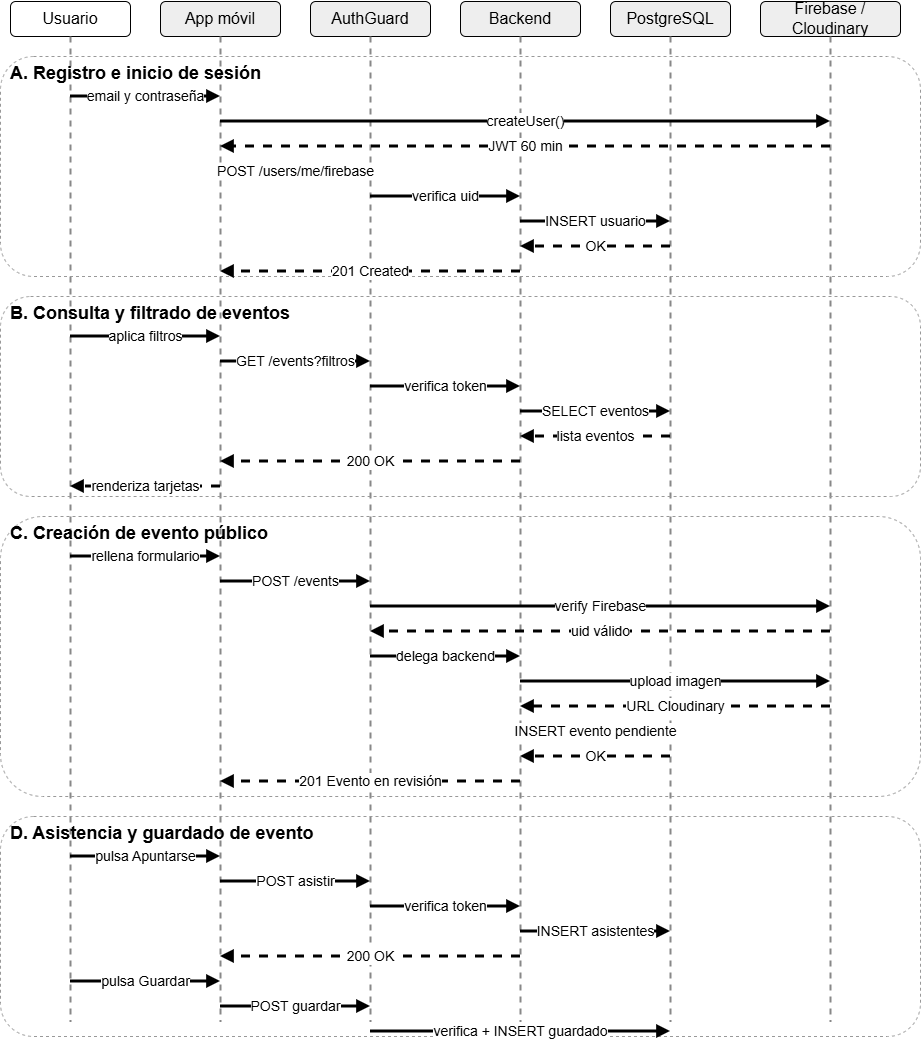
\includegraphics[width=\textwidth]{figures/secuencias_usuario.png}
\caption{Diagrama de secuencias del flujo del usuario (registro, consulta, creación y asistencia)}
\label{fig:seq_usuario}
\end{figure}

% ═══════════════════════════════════════════════════════════════
\section{Diseño del sistema de moderación}

La moderación de eventos públicos es una de las piezas centrales del sistema. El moderador accede al panel de moderación, revisa los eventos en estado \textbf{Pendiente}, puede editarlos directamente antes de tomar una decisión, y los aprueba o rechaza. Además, dispone de un listado independiente con los eventos públicos, que puede editar o eliminar si detecta errores, información desactualizada o contenido inadecuado. La notificación correspondiente se envía al creador cuando el evento pendiente se aprueba o rechaza. La figura~\ref{fig:seq_moderador} muestra este flujo.

\begin{figure}[H]
\centering
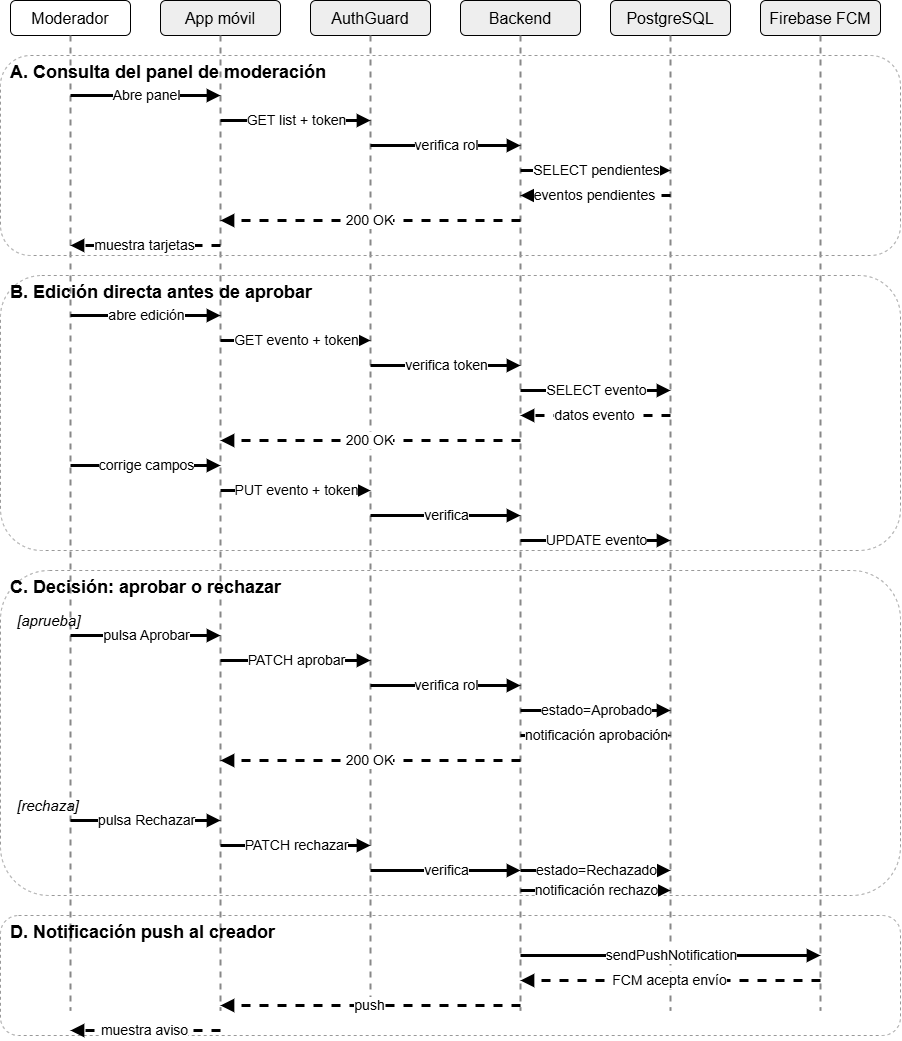
\includegraphics[width=\textwidth]{figures/secuencias_moderador.png}
\caption{Diagrama de secuencias del flujo del moderador}
\label{fig:seq_moderador}
\end{figure}

El ciclo de vida de un evento depende principalmente de su visibilidad:

\begin{itemize}
    \item \textbf{Eventos públicos}: al crearse quedan en estado \textbf{Pendiente}. No se muestran en el listado general ni en el listado de edición del usuario mientras esperan revisión. El moderador puede corregirlos si detecta errores menores y después aprobarlos o rechazarlos. Si se aprueban, pasan a estado \textbf{Aprobado} y aparecen en la aplicación; si se rechazan, dejan de estar disponibles para los usuarios.
    \item \textbf{Eventos privados}: no pasan por moderación. Se crean directamente como \textbf{Aprobados} y solo son accesibles mediante su enlace de invitación. El botón de compartir se sustituye por la acción \textit{invitar}, disponible únicamente para el creador del evento.
    \item \textbf{Ediciones de eventos públicos}: cuando el creador modifica un evento público ya aprobado, el evento vuelve a estado \textbf{Pendiente} y deja de mostrarse hasta que el moderador revise los cambios. Si la modificación la realiza un moderador desde su panel, el evento conserva el estado \textbf{Aprobado}.
    \item \textbf{Cambios de visibilidad}: si un evento privado pasa a público, entra en moderación como \textbf{Pendiente}. Si un evento público pasa a privado, se aprueba automáticamente y se genera un enlace de acceso.
\end{itemize}

El panel de moderación separa dos tareas: por un lado, la revisión de eventos pendientes; por otro, la supervisión de eventos públicos ya aprobados. Esto permite que el moderador apruebe o rechace nuevo contenido, pero también corrija o elimine eventos públicos que hayan quedado desactualizados o contengan información incorrecta.

% ═══════════════════════════════════════════════════════════════
\section{Flujo de interacción del administrador}

El administrador gestiona la estructura del sistema: consulta el listado de usuarios, cambia sus roles y administra las categorías de eventos. No interviene en el flujo de moderación de contenido. La figura~\ref{fig:seq_admin} muestra estas interacciones.

\begin{figure}[H]
\centering
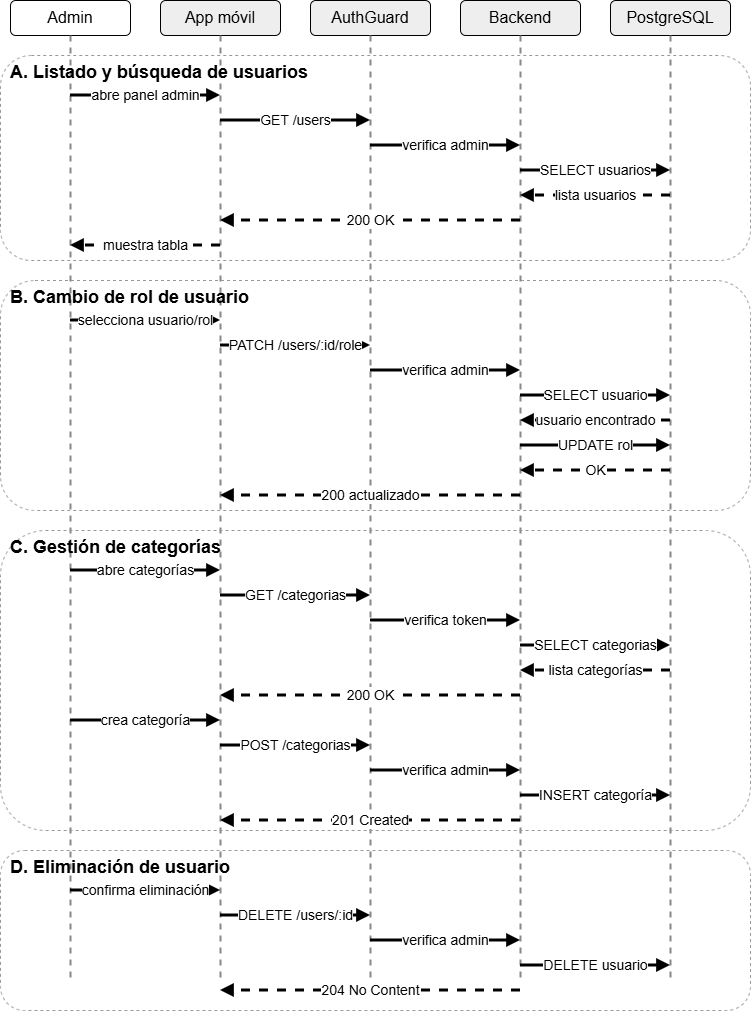
\includegraphics[width=\textwidth]{figures/secuencias_admin.png}
\caption{Diagrama de secuencias del flujo del administrador}
\label{fig:seq_admin}
\end{figure}

\section{Diseño de la interfaz de usuario}

\subsection{Principios de diseño}

La interfaz de usuario ha sido diseñada siguiendo los principios de usabilidad para aplicaciones móviles:

\begin{itemize}
    \item \textbf{Consistencia visual}: se utiliza un sistema de componentes temáticos (\texttt{ThemedView}, \texttt{ThemedCard}, \texttt{ThemedButton}, \texttt{ThemedText}) que garantizan una apariencia coherente en todas las pantallas, tanto en modo claro como en modo oscuro.
    \item \textbf{Adaptabilidad}: la aplicación soporta modo claro y modo oscuro, adaptándose automáticamente a la preferencia del sistema o permitiendo el cambio manual desde el perfil.
    \item \textbf{Jerarquía de información}: cada pantalla prioriza la información más relevante para el usuario, ocultando las opciones avanzadas o de administración según el rol.
    \item \textbf{Accesibilidad de acciones}: las acciones principales (apuntarse, guardar, compartir) están siempre visibles en el detalle de evento sin necesidad de desplazarse.
\end{itemize}

\subsection{Grafo de navegación}

La aplicación se divide en dos grupos de pantallas según el estado de autenticación del usuario. La figura~\ref{fig:grafo_navegacion} muestra el grafo de navegación completo.

\begin{figure}[H]
\centering
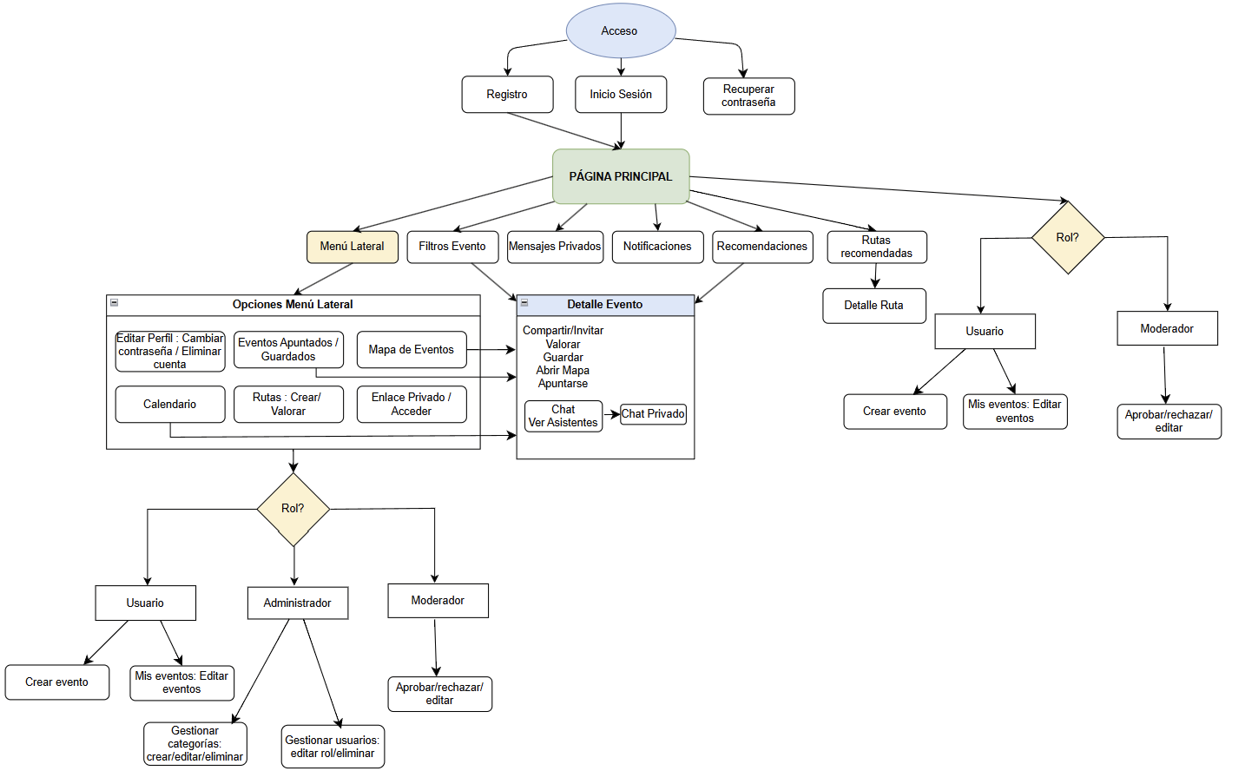
\includegraphics[width=\textwidth,height=0.78\textheight,keepaspectratio]{figures/grafo_navegacion.png}
\caption{Grafo de navegación de la aplicación organizado por rol de acceso}
\label{fig:grafo_navegacion}
\end{figure}

El grupo de pantallas no autenticadas comprende las pantallas de inicio de sesión, registro y política de privacidad. El grupo de pantallas autenticadas incluye todas las funcionalidades de la aplicación, organizadas alrededor de la pantalla principal.

Las pantallas exclusivas de moderador y administrador solo son accesibles si el usuario dispone del rol correspondiente; de lo contrario, no aparecen en el menú lateral ni en ningún punto de entrada de la navegación.

\subsection{Pantallas del sistema}

La tabla~\ref{tab:pantallas} describe las pantallas del sistema y su accesibilidad según el rol del usuario.

{\renewcommand{\arraystretch}{1.2}
\begin{longtable}{|
>{\raggedright\arraybackslash}p{0.23\textwidth}|
>{\raggedright\arraybackslash}p{0.51\textwidth}|
>{\raggedright\arraybackslash}p{0.18\textwidth}|}
\caption{Pantallas del sistema y roles que pueden acceder}
\label{tab:pantallas}\\
\hline
\textbf{Pantalla} & \textbf{Descripción} & \textbf{Acceso} \\
\hline
\endfirsthead
\hline
\textbf{Pantalla} & \textbf{Descripción} & \textbf{Acceso} \\
\hline
\endhead
Inicio de sesión & Autenticación con correo y contraseña & No autenticado \\
\hline
Registro & Creación de cuenta nueva & No autenticado \\
\hline
Pantalla principal & Listado de eventos con filtros y recomendaciones & Todos los roles \\
\hline
Detalle de evento & Información completa, chat, reseñas y asistencia & Todos los roles \\
\hline
Mapa de eventos & Vista cartográfica de los eventos cercanos & Todos los roles \\
\hline
Calendario & Eventos con fecha a los que está apuntado el usuario & Todos los roles \\
\hline
Acceso a evento privado & Acceso a evento privado mediante enlace de invitación & Todos los roles \\
\hline
Guardados y privados & Eventos guardados y eventos privados del usuario & Todos los roles \\
\hline
Crear evento & Formulario de creación de evento público o privado & Usuario \\
\hline
Editar evento & Modificación de un evento propio & Usuario creador \\
\hline
Mis eventos & Listado de eventos creados por el usuario & Usuario \\
\hline
Rutas & Listado de rutas públicas & Todos los roles \\
\hline
Detalle de ruta & Información de la ruta y secuencia de eventos & Todos los roles \\
\hline
Rutas recomendadas & Itinerarios generados automáticamente para el usuario & Todos los roles \\
\hline
Vista previa de ruta & Previsualización de una ruta recomendada & Todos los roles \\
\hline
Crear ruta & Formulario para crear una ruta propia & Todos los roles \\
\hline
Notificaciones & Listado de notificaciones del usuario & Todos los roles \\
\hline
Mensajes & Lista de conversaciones privadas & Todos los roles \\
\hline
Mensaje directo & Chat privado entre dos usuarios & Todos los roles \\
\hline
Perfil de usuario & Vista del perfil de otro usuario, con acciones sociales y eventos a los que asiste & Todos los roles \\
\hline
Amigos & Módulo social con búsqueda de usuarios, seguidores, seguidos y amistades mutuas & Todos los roles \\
\hline
Conexiones & Listado de seguidores y seguidos de un usuario concreto & Todos los roles \\
\hline
Editar perfil & Modificación de datos personales e intereses & Todos los roles \\
\hline
Cambiar contraseña & Modificación de la contraseña de la cuenta & Todos los roles \\
\hline
Panel de administración & Estadísticas globales, gestión de usuarios, roles y scraping & Administrador \\
\hline
Gestión de categorías & Creación, edición y eliminación de categorías & Administrador \\
\hline
Moderación de eventos & Revisión y aprobación de eventos pendientes & Moderador \\
\hline
Edición moderada & Edición directa de un evento pendiente antes de aprobarlo & Moderador \\
\hline
Ayuda & Preguntas frecuentes y guía de uso de la aplicación & Todos los roles \\
\hline
Política de privacidad & Política de tratamiento de datos personales & Todos \\
\hline
Atribuciones legales & Licencias y atribuciones de recursos de terceros & Todos los roles \\
\hline
\end{longtable}}


\section{Diseño del sistema de comunicación en tiempo real}

El chat de la aplicación está implementado sobre \textbf{Socket.IO}~\cite{socketio}, integrado en el mismo servidor NestJS que la API REST. Se definen dos canales de comunicación independientes:

\begin{itemize}
    \item \textbf{Chat de evento}: sala identificada por \texttt{event:\{eventId\}} en la que todos los asistentes pueden leer y enviar mensajes.
    \item \textbf{Mensajes privados}: sala personal identificada por \texttt{user:\{userId\}} que enruta los mensajes directos entre dos usuarios.
\end{itemize}

La conexión WebSocket se autentica con el mismo token de Firebase que los endpoints REST, verificado en el middleware del socket antes de aceptar la conexión. Para prevenir el abuso, el servidor aplica un límite de 10 mensajes por ventana de 10 segundos por conexión.

\subsection{Ciclo de vida de la conexión y los listeners}

La conexión WebSocket se centraliza en el \texttt{SocketProvider}. Cuando la aplicación se monta con una sesión activa, el proveedor abre una única conexión Socket.IO autenticada con el token de Firebase y la comparte con el resto de pantallas mediante el contexto de React. La conexión se cierra al desmontarse el proveedor o si pasan 24 horas sin que el cliente envíe mensajes a través de \texttt{sendMessage}; cada envío reinicia ese temporizador.

Los \textit{listeners} no se registran de forma global, sino en las pantallas que los necesitan. En el detalle de un evento se emite \texttt{join\_room} para entrar en la sala del evento y se registran listeners como \texttt{chat\_history}, \texttt{chat\_message}, \texttt{delete\_event\_message\_success} y \texttt{chat\_error}. En el chat privado se solicita el historial con \texttt{dm\_history} y se escuchan \texttt{dm\_history}, \texttt{dm\_message} y \texttt{delete\_dm\_success}. Las pantallas que muestran conversaciones emiten \texttt{get\_conversations} y escuchan eventos como \texttt{conversations}, \texttt{refresh\_conversations} y \texttt{dm\_message}.

Al salir de estas pantallas, el cleanup de sus \texttt{useEffect} elimina los listeners con \texttt{socket.off()}. Así se reutiliza la misma conexión durante la navegación, pero se evita acumular manejadores duplicados al entrar y salir de chats o conversaciones.

La figura~\ref{fig:flujo_socket} muestra el flujo completo desde el establecimiento de la conexión hasta la recepción del mensaje en otro cliente.

\begin{figure}[H]
\centering
\begin{tikzpicture}[
    node distance=0.85cm and 2.0cm,
    every node/.style={font=\small},
    box/.style={draw, rounded corners=3pt, minimum width=3.2cm, minimum height=0.7cm, align=center, fill=white},
    ext/.style={draw, rounded corners=3pt, minimum width=3.0cm, minimum height=0.7cm, align=center, fill=gray!12},
    arr/.style={-{Stealth[length=5pt]}, thick},
    darr/.style={{Stealth[length=5pt]}-{Stealth[length=5pt]}, thick, dashed},
]
\node[box] (clientA) {Cliente A\\(app móvil)};
\node[box, below=of clientA]  (ctxA)   {SocketContext};
\node[box, below=of ctxA]     (mid)    {Middleware Socket.IO\\(verifica token Firebase)};
\node[box, below=of mid]      (gate)   {ChatGateway (NestJS)};
\node[box, below=of gate]     (svcMsg) {MensajesService};
\node[box, below=of svcMsg]   (db)     {PostgreSQL};

\node[box, right=3.2cm of gate]   (sala)   {Sala: event:\{id\}\\o user:\{id\}};
\node[box, right=3.2cm of ctxA]   (clientB){Cliente B\\(app móvil)};

\node[ext, left=2.6cm of mid]    (fbadm)  {Firebase Admin SDK};

% Flechas verticales izquierda
\draw[arr] (clientA) -- node[right, font=\tiny] {connect(token)} (ctxA);
\draw[arr] (ctxA)    -- node[right, font=\tiny] {WS handshake} (mid);
\draw[arr] (mid)     -- node[right, font=\tiny] {conexión aceptada} (gate);
\draw[arr] (gate)    -- node[right, font=\tiny] {persiste} (svcMsg);
\draw[arr] (svcMsg)  -- node[right, font=\tiny] {INSERT} (db);

% Verificación token
\draw[arr] (mid) -- node[above, font=\tiny] {verifyIdToken()} (fbadm);

% Sala y emit
\draw[arr] (gate) -- node[above, font=\tiny] {join room} (sala);
\draw[arr] (sala.north) -- node[right, font=\tiny] {emit evento} (clientB.south);
\end{tikzpicture}
\caption{Flujo de comunicación en tiempo real mediante Socket.IO: conexión, autenticación y entrega de mensajes}
\label{fig:flujo_socket}
\end{figure}

\section{Diseño del sistema de recomendaciones}

El motor de recomendaciones es un componente del backend que genera listas de eventos personalizadas para cada usuario. Su diseño se basa en un algoritmo de puntuación multifactorial~\cite{ricci2015recommender}: cada evento candidato recibe una puntuación calculada como suma ponderada de varios factores relacionados con el comportamiento del usuario, sus intereses declarados, la proximidad temporal y la proximidad geográfica.

Los factores con mayor peso en el diseño son la afinidad por categoría (hasta 12 puntos), el haber guardado previamente el evento (+10) y la proximidad temporal al evento (hasta 8 puntos). Los eventos se ordenan de mayor a menor puntuación y se devuelven los más relevantes.

Cabe destacar que este algoritmo de \textit{scoring} multifactorial no es un patrón de diseño de software en el sentido estructural o de comportamiento (GoF), sino un algoritmo de dominio propio del problema de recomendación. Su característica clave es que cada factor es independiente y ponderado: modificar el peso de un criterio o incorporar uno nuevo no afecta al cálculo del resto, lo que facilita su ajuste y extensión.

La figura~\ref{fig:flujo_recomendaciones} muestra las entradas que consulta el motor y el proceso de puntuación hasta producir la lista final.

\begin{figure}[H]
\centering
\begin{tikzpicture}[
    node distance=0.8cm and 1.6cm,
    every node/.style={font=\small},
    box/.style={draw, rounded corners=3pt, minimum width=3.2cm, minimum height=0.7cm, align=center, fill=white},
    input/.style={draw, rounded corners=3pt, minimum width=2.8cm, minimum height=0.65cm, align=center, fill=gray!10},
    arr/.style={-{Stealth[length=5pt]}, thick},
]
% Entradas
\node[input] (u1) {Intereses del usuario\\(categorías)};
\node[input, below=of u1] (u2) {Eventos asistidos\\y guardados};
\node[input, below=of u2] (u3) {Ubicación del usuario\\(punto PostGIS)};
\node[input, below=of u3] (u4) {Fecha actual};

% Motor
\node[box, right=2.6cm of u2] (motor) {Motor de puntuación\\multifactorial};

% Salida
\node[box, right=2.4cm of motor] (rank)  {Lista ordenada\\por puntuación};
\node[box, above=of rank]        (evtos) {Eventos candidatos\\(PostgreSQL)};

\draw[arr] (u1) -- (motor);
\draw[arr] (u2) -- (motor);
\draw[arr] (u3) -- (motor);
\draw[arr] (u4) -- (motor);
\draw[arr] (evtos) -- (motor);
\draw[arr] (motor) -- (rank);
\end{tikzpicture}
\caption{Entradas y proceso del motor de recomendaciones}
\label{fig:flujo_recomendaciones}
\end{figure}

El mismo motor puede generar rutas recomendadas aplicando tres estrategias seleccionables:

\begin{itemize}
    \item \textbf{balanced}: equilibra puntuación y distancia recorrida entre eventos.
    \item \textbf{walkable}: minimiza la distancia total del itinerario.
    \item \textbf{score}: maximiza la puntuación agregada de los eventos incluidos.
\end{itemize}

\section{Patrones de diseño aplicados}

A lo largo del desarrollo de \textbf{Sevillaneando} se han aplicado varios patrones de diseño reconocidos~\cite{gamma1994design}, algunos inherentes a los frameworks elegidos y otros aplicados de forma deliberada. La tabla~\ref{tab:patrones} resume los más relevantes.

\begin{table}[H]
\centering
\caption{Patrones de diseño aplicados en el sistema}
\label{tab:patrones}
\renewcommand{\arraystretch}{1.2}
\begin{tabular}{|
>{\raggedright\arraybackslash}p{0.16\textwidth}|
>{\raggedright\arraybackslash}p{0.25\textwidth}|
>{\raggedright\arraybackslash}p{0.49\textwidth}|}
\hline
\textbf{Patrón} & \textbf{Dónde se aplica} & \textbf{Por qué} \\
\hline
Módulo & Backend NestJS & Cada dominio (\textit{EventosModule}, \textit{UsuariosModule}, etc.) encapsula controlador, servicio y entidades. Facilita el mantenimiento y la extensión sin afectar a otros módulos. \\
\hline
Repositorio & TypeORM & Los servicios acceden a la base de datos a través de repositorios tipados, desacoplando la lógica de negocio del SQL y permitiendo sustituirlos por dobles en pruebas unitarias. \\
\hline
Guard & \texttt{FirebaseAuthGuard}, \texttt{RolesGuard} & Centraliza la autenticación y la autorización interceptando cada petición antes del controlador, evitando duplicar esa lógica en cada endpoint. \\
\hline
Interceptor & Cliente Axios (frontend) & Inyecta automáticamente el token Firebase en cada petición y aplica reintentos ante errores de red, sin repetir esa lógica en cada llamada al servicio. \\
\hline
Contexto / Proveedor & \texttt{AuthContext}, \texttt{SocketContext}, \texttt{ThemeContext}, \texttt{Notificaciones\allowbreak{}Context} & Gestiona el estado global del frontend evitando \textit{prop drilling}. La separación en cuatro contextos independientes evita rerenders innecesarios entre dominios. \\
\hline
Estrategia & \texttt{IScraper} & Cada fuente externa implementa la misma interfaz; el orquestador trabaja con la abstracción. Permite añadir nuevas fuentes sin modificar la lógica de orquestación. \\
\hline
Observador & Socket.IO (chat) & El servidor emite eventos a las salas y los clientes suscritos los reciben automáticamente, desacoplando al emisor del receptor. \\
\hline
Estado & Flujo de moderación de eventos & El ciclo de vida del evento (\texttt{Pendiente} → \texttt{Aprobado} / \texttt{Rechazado}) tiene transiciones controladas; no todas son válidas, lo que garantiza la coherencia del flujo. \\
\hline
\end{tabular}
\end{table}

\section{Decisiones de diseño relevantes}

A lo largo del proceso de diseño se tomaron una serie de decisiones que merecen una justificación explícita, ya que no son evidentes a partir de los requisitos y condicionan la arquitectura y el comportamiento de la aplicación.

\subsection{Roles, permisos y responsabilidades}

Este bloque agrupa las decisiones relacionadas con el reparto de responsabilidades entre usuario, moderador y administrador, así como con las operaciones que pueden afectar al contenido creado por otros usuarios.

\subsubsection{Por qué tres roles y no más ni menos}

El sistema define tres roles: \textbf{usuario}, \textbf{moderador} y \textbf{administrador}. Esta jerarquía mínima responde a la necesidad de separar tres tipos de responsabilidad claramente diferenciados:

\begin{itemize}
    \item El \textbf{usuario} es el actor principal del sistema: crea, consulta y consume contenido. No tiene autoridad sobre el contenido de otros ni sobre la configuración del sistema.
    \item El \textbf{moderador} actúa como filtro de calidad: revisa y valida eventos antes de que sean visibles públicamente, y también puede editar eventos públicos cuando sea necesario corregir o completar su información. Requiere más permisos que un usuario ordinario, pero no debe tener acceso a la gestión del sistema, lo que delimita claramente su responsabilidad.
    \item El \textbf{administrador} gestiona la estructura del sistema (roles y categorías) pero no interviene en el contenido concreto. Esta separación evita que una única persona acumule tanto la capacidad de gestionar usuarios como la de aprobar contenido, reduciendo el riesgo de abusos y errores.
\end{itemize}

Añadir más roles (por ejemplo, un \textit{superadmin} o un \textit{editor}) habría incrementado la complejidad de la gestión de permisos sin aportar valor real al caso de uso concreto de la aplicación. Un único rol con todos los permisos habría eliminado la separación de responsabilidades que protege la integridad del contenido y del sistema.

\subsubsection{Por qué la eliminación de eventos es explícita y restringida}

La eliminación de eventos se realiza mediante el endpoint \texttt{DELETE /events/\{id\}}, protegido con autenticación Firebase. Aunque el endpoint no declara un rol concreto en el controlador, el servicio vuelve a comprobar los permisos antes de borrar: el creador puede eliminar sus propios eventos, y los usuarios con rol de moderador o administrador solo pueden eliminar eventos que no sean privados. Por tanto, no es una acción automática ni accesible para cualquier usuario autenticado.

\begin{itemize}
    \item \textbf{Control de autoría}: el creador conserva la capacidad de retirar un evento propio que ya no desea mantener publicado o accesible.
    \item \textbf{Control de calidad}: el moderador puede eliminar eventos no privados cuando detecta contenido inadecuado, duplicado o incorrecto.
    \item \textbf{Reducción de riesgo}: los eventos privados ajenos quedan fuera del alcance de moderadores y administradores para preservar su naturaleza restringida.
\end{itemize}

En la interfaz, la eliminación aparece en la pantalla de edición del creador y en la pantalla de edición de moderación, siempre con confirmación previa. Al ejecutarse, el backend elimina primero relaciones asociadas al evento, como asistentes, mensajes y reseñas, y después borra el propio evento.

\subsection{Moderación y ciclo de vida de eventos}

Las siguientes decisiones explican cómo se conserva el historial de eventos, cómo intervienen moderadores y administradores y qué reglas evitan que el contenido publicado dependa de acciones automáticas poco transparentes.

\subsubsection{Por qué los eventos finalizados no se borran}

Un evento finalizado sigue teniendo valor informativo y social dentro del sistema:

\begin{itemize}
    \item Los usuarios que asistieron pueden seguir leyendo el chat del evento y las reseñas dejadas por otros asistentes.
    \item Las reseñas escritas sobre el evento permanecen accesibles y contribuyen a la reputación del creador del evento.
    \item Las rutas que incluyen ese evento mantienen su coherencia: una ruta cultural puede referenciar un evento ya celebrado como parte del itinerario.
    \item El historial de eventos pasados permite al motor de recomendaciones analizar patrones de asistencia y mejorar las sugerencias futuras.
\end{itemize}

Borrar eventos finalizados de forma automática habría reducido la utilidad histórica y social del sistema sin beneficio claro para el usuario.

\subsubsection{Por qué el moderador puede editar un evento directamente antes de aprobarlo}

El rol del moderador no se limita a aprobar o rechazar: puede detectar que un evento tiene un error menor (fecha incorrecta, descripción incompleta, categoría equivocada) que no justifica el rechazo completo. Rechazar ese evento obliga al creador a corregirlo y volver a someterlo a moderación, lo que genera fricción innecesaria.

La pantalla de edición moderada permite al moderador corregir directamente los campos necesarios y publicar el evento en un único paso. Esto:

\begin{itemize}
    \item Reduce el número de ciclos de moderación para eventos con errores menores.
    \item Agiliza la publicación de contenido de calidad sin depender de la disponibilidad del creador para aplicar los cambios.
    \item Concentra en el moderador la responsabilidad de garantizar que el contenido publicado cumple los estándares del sistema.
\end{itemize}

\subsubsection{Por qué el administrador gestiona la configuración y la operación del sistema}

El administrador tiene un alcance orientado a la configuración y operación general de la plataforma. Desde la aplicación puede consultar estadísticas globales, gestionar usuarios y roles, administrar las categorías de eventos y restablecer los eventos procedentes del sistema de scraping. En cambio, no participa en la revisión diaria del contenido desde el flujo principal de moderación. Esta separación es deliberada:

\begin{itemize}
    \item \textbf{Separación de poderes}: el administrador configura quién puede hacer qué y mantiene los datos estructurales del sistema, pero la revisión habitual de eventos queda delegada en el moderador.
    \item \textbf{Supervisión operativa}: el panel de estadísticas permite conocer el estado global de la plataforma, incluyendo usuarios registrados, eventos por estado y eventos obtenidos mediante scraping.
    \item \textbf{Mantenimiento del scraping}: el restablecimiento del scraping permite eliminar y regenerar eventos importados automáticamente cuando las fuentes externas cambian o se necesita refrescar el catálogo.
    \item \textbf{Principio de mínimo privilegio}: aunque el administrador dispone de permisos técnicos amplios, la interfaz separa sus tareas de gestión y mantenimiento de las tareas editoriales propias del moderador.
\end{itemize}

\subsection{Comunicación, tiempo real y notificaciones}

Este bloque reúne las decisiones relacionadas con el chat, la conexión WebSocket y las notificaciones generadas automáticamente.

\subsubsection{Por qué el chat incluye persistencia y no es solo en tiempo real}

El chat de evento está implementado con \textbf{Socket.IO} para la transmisión en tiempo real, pero todos los mensajes se persisten en base de datos (entidades \texttt{Mensaje} y \texttt{MensajePrivado}). Esta decisión responde a dos necesidades diferenciadas: el valor social del chat antes y durante el evento, y su utilidad después de que este haya terminado.

Antes y durante el evento, el chat es el espacio donde los asistentes pueden coordinarse: quedar para ir juntos, resolver dudas sobre el lugar o el horario, compartir fotos o simplemente conocer a otras personas que van al mismo plan. Para que esto sea posible, el historial debe estar disponible para cualquiera que se una al chat más tarde; sin persistencia, quien llegara después solo vería el estado actual de la conversación y perdería todo el contexto previo. Lo mismo aplica a los mensajes privados: si el receptor no está conectado en el momento del envío, el mensaje se perdería sin persistencia.

Después del evento, el chat conserva el mismo valor que el resto del historial del evento: otros usuarios pueden consultar la conversación para saber cómo fue, qué opinaron los asistentes o si merece la pena acudir a futuras ediciones. Esto conecta directamente con las razones por las que los eventos tampoco se eliminan del sistema.

\subsubsection{Por qué las notificaciones programadas se separan en tres métodos}

El sistema no define tres clases scheduler independientes, sino una clase \texttt{NotificacionesScheduler} con tres métodos diferenciados. Cada método cubre un caso de notificación distinto: eventos cercanos en el espacio (radio de 1 km), eventos próximos en el tiempo (7 días) y eventos con menos de 24 horas. El endpoint \texttt{POST /scheduler/run-notifications} ejecuta los tres métodos de forma conjunta, pero la lógica permanece separada para que cada criterio pueda revisarse, probarse y modificarse de forma independiente.

\subsubsection{Por qué la conexión WebSocket se autentica en el \textit{handshake} y no por mensaje}

La autenticación del socket se realiza en el middleware de conexión de Socket.IO, antes de que se establezca la sala y se procese cualquier mensaje. Si la autenticación fallara por mensaje (es decir, si se aceptara la conexión y se verificara el token en el primer evento recibido), existiría una ventana de tiempo en la que un cliente no autenticado tendría una conexión activa y podría enviar eventos al servidor. Verificar en el \textit{handshake} garantiza que ninguna conexión sin token válido llega a establecerse, simplificando además la lógica de cada handler de eventos, que puede asumir que el socket ya está autenticado.

\subsubsection{Por qué el historial de chat se limita a los últimos 50 mensajes}

Al incorporarse a la sala de chat de un evento, el servidor envía al cliente los últimos 50 mensajes almacenados. Un límite superior habría aumentado el tamaño del payload inicial y el tiempo de carga de la pantalla de detalle de evento, especialmente en eventos con chats muy activos. Un límite inferior habría privado al usuario de contexto suficiente para entender la conversación reciente. El valor de 50 mensajes representa un equilibrio razonable entre utilidad y rendimiento para el caso de uso típico de la aplicación.

\subsection{Visibilidad, recurrencia y datos geográficos}

Este bloque recoge las decisiones que afectan a la forma en que se publican, comparten y consultan los eventos dentro del modelo de datos.

\subsubsection{Por qué los eventos privados se aprueban automáticamente}

Cuando un usuario crea un evento privado, el sistema le asigna directamente el estado \textbf{Aprobado} sin pasar por el flujo de moderación. La razón es que los eventos privados no son visibles en el listado público: solo acceden a ellos las personas que disponen del enlace de invitación. El objetivo de la moderación es garantizar la calidad del contenido que el público en general puede encontrar; un evento cuyo alcance está restringido a las personas que el creador decide invitar no supone un riesgo para la comunidad y no requiere revisión externa.

Someter los eventos privados a moderación habría generado una experiencia confusa: el creador crearía un evento para compartir con amigos y tendría que esperar aprobación antes de poder enviar el enlace. Esta fricción no se corresponde con el modelo de uso esperado.

\subsubsection{Por qué los eventos privados usan un enlace UUID en lugar de una lista de control de acceso}

El acceso a eventos privados se implementa mediante un enlace único generado automáticamente (UUID v4) en lugar de una lista explícita de usuarios autorizados. Esta decisión responde a varias consideraciones:

\begin{itemize}
    \item \textbf{Simplicidad de uso}: el creador puede compartir el enlace por cualquier canal externo (mensaje, correo, red social) sin necesidad de que los invitados tengan cuenta en la aplicación o deban ser añadidos manualmente.
    \item \textbf{Flexibilidad}: el creador decide el canal y el momento del reparto sin intervención del sistema.
    \item \textbf{Sin fricción para el invitado}: no se requiere autenticación para acceder al detalle del evento por enlace, lo que facilita que alguien consulte los datos antes de registrarse.
\end{itemize}

La contrapartida es que quien obtiene el enlace puede reenviarlo. Este riesgo es aceptable en el contexto de la aplicación, ya que los eventos privados son de naturaleza social e informal.

\subsubsection{Por qué los eventos recurrentes generan instancias independientes en base de datos}

Cuando se crea un evento con recurrencia (diaria, semanal, quincenal o mensual), el sistema genera un registro independiente en base de datos por cada ocurrencia hasta la fecha de fin de recurrencia. La alternativa habría sido almacenar una regla de recurrencia única y calcular las ocurrencias en tiempo de consulta.

Se eligió la generación de instancias por las siguientes razones:

\begin{itemize}
    \item Cada instancia puede tener su propio estado de moderación, chat, reseñas y lista de asistentes de forma independiente. Con una regla única esto sería mucho más complejo de gestionar.
    \item Las consultas espaciales y temporales de PostGIS operan sobre registros concretos. Calcular ocurrencias en tiempo de consulta habría requerido lógica adicional dentro de las queries geoespaciales, complicando el motor de filtrado.
    \item La coherencia con el resto del modelo de datos es total: una instancia recurrente es un evento como cualquier otro para el resto del sistema (recomendaciones, rutas, notificaciones).
\end{itemize}

La desventaja es que la base de datos crece proporcionalmente al número de ocurrencias generadas, pero dado el alcance de la aplicación este coste es despreciable.

\subsubsection{Por qué se usa PostGIS con tipo \textit{geography} y SRID 4326}

Las ubicaciones de usuarios y eventos se almacenan como puntos \texttt{geography} de PostGIS con sistema de referencia SRID 4326 (WGS84), que es el mismo sistema que utilizan el GPS y la mayoría de servicios cartográficos. Se eligió el tipo \texttt{geography} frente al tipo \texttt{geometry} porque \texttt{geography} trabaja directamente en coordenadas esféricas: las funciones \texttt{ST\_DWithin} y \texttt{ST\_Distance} devuelven distancias en metros sin necesidad de reproyectar, lo que simplifica las consultas de filtrado por radio y elimina el error de distorsión que aparece con \texttt{geometry} en coordenadas geográficas.

La alternativa de almacenar latitud y longitud como dos columnas numéricas habría impedido aprovechar los índices espaciales de PostGIS (GIST), lo que habría degradado significativamente el rendimiento de las consultas de filtrado por proximidad a medida que crece el número de eventos.

\subsection{Automatización y fuentes externas}

Las siguientes decisiones justifican cómo se obtienen eventos desde fuentes externas y cómo se planifican las tareas periódicas fuera de la interacción directa del usuario.

\subsubsection{Por qué el scraping se ejecuta a las 3:00 AM}

La tarea de obtención de eventos externos (Eventbrite, Ticketmaster y webs institucionales y de ocio procesadas con Gemini AI) se programa a las 3:00 AM mediante un \textit{cron job} diario. Esta hora se eligió porque es el período de menor actividad de usuarios en la aplicación, lo que reduce la competencia por recursos del servidor y de la base de datos durante el proceso de scraping. Además, ejecutarlo una vez al día es suficiente para mantener el catálogo actualizado: los eventos de ocio y cultura no cambian con frecuencia mayor a la diaria.

\subsubsection{Por qué el cron job es externo y no interno al backend}

La planificación de las tareas periódicas (scraping diario y envío de notificaciones) se gestiona mediante un servicio de \textit{cron} externo (cron-job.org) que invoca los endpoints \texttt{POST /scheduler/run-scraping} y \texttt{POST /scheduler/run-notifications}, en lugar de usar el planificador interno de NestJS (\texttt{@nestjs/schedule}).

La razón principal es la infraestructura de despliegue: el backend se aloja en Render con el plan gratuito, que suspende el proceso tras 15 minutos de inactividad. Cuando el proceso está suspendido, el planificador interno de NestJS no corre; y cuando Render lo reactiva ante una nueva petición, el planificador se reinicia desde cero. Esto hace que los \texttt{@Cron} internos sean poco fiables: la tarea diaria de las 3:00 AM o la de notificaciones horarias podrían no ejecutarse si el proceso lleva inactivo más de 15 minutos antes de la hora programada.

Un \textit{cron} externo es independiente del ciclo de vida del proceso del servidor: aunque el backend esté suspendido, la petición del \textit{cron} externo lo reactiva y ejecuta la tarea. Además, el servicio de \textit{keep-alive} (que llama periódicamente a \texttt{GET /scheduler/health}) se gestiona también desde el mismo sistema externo, lo que centraliza en un único panel el control de todas las tareas programadas y su historial de ejecuciones.

El \textit{cron} interno de NestJS sería la opción preferida si el backend corriera de forma continua en un servidor dedicado o en un plan de pago con instancias siempre activas: en ese caso eliminaría la dependencia de un servicio externo y la latencia de la petición HTTP entrante. Para el contexto actual de la aplicación, con infraestructura gratuita, el \textit{cron} externo es la solución más fiable.

\subsubsection{Por qué los scrapers siguen el patrón estrategia con interfaz \texttt{IScraper}}

Cada fuente de eventos externos (Eventbrite, Ticketmaster, Visita Sevilla y webs institucionales y de ocio de Sevilla procesadas con Gemini AI) está implementada como un scraper independiente que implementa la interfaz \texttt{IScraper}. Esto permite añadir nuevas fuentes de datos sin modificar la lógica de orquestación del servicio de scraping. La alternativa de implementar el scraping como código monolítico habría acoplado la lógica de cada fuente con el proceso de guardado en base de datos, dificultando el mantenimiento cuando alguna de las fuentes externas cambia su estructura.

Además, todos los eventos scraped se asignan a un único usuario técnico del sistema (\textit{scraper-bot}), centralizado con un UID y correo fijos. Esto simplifica la trazabilidad: es inmediato identificar qué eventos provienen de fuentes externas y quién es su ``creador'' a efectos del modelo de datos.

\subsubsection{Por qué se ha implementado scraping en lugar de usar únicamente APIs oficiales}

El contenido de eventos de la aplicación proviene de dos grandes bloques: eventos creados por usuarios y eventos obtenidos automáticamente de fuentes externas. Para estas últimas se utilizan cuatro estrategias complementarias:

\begin{itemize}
    \item \textbf{Scraping HTML con JSON-LD (Eventbrite)}: el \texttt{SevillaScraperService} descarga la página de eventos de Sevilla en Eventbrite mediante \texttt{axios} y parsea el HTML con \texttt{cheerio}, extrayendo tarjetas de eventos y bloques JSON-LD estructurados embebidos en la página.
    \item \textbf{API oficial de Ticketmaster}: el \texttt{TicketmasterScraperService} consume la API Discovery de Ticketmaster paginando resultados en bloques de hasta 100 eventos, filtrando por ciudad y fecha.
    \item \textbf{Scraping dedicado de Visita Sevilla}: el \texttt{VisitaSevillaScraperService} descarga la agenda de \texttt{visitasevilla.es} y parsea su HTML con \texttt{cheerio}. Se ha implementado un scraper específico porque la web utiliza un formato de fecha propio (\texttt{DD.MM.YY} y rangos \texttt{DD.MM.YY-DD.MM.YY}) que no puede interpretarse correctamente mediante extracción genérica con IA. El scraper descarta los placeholders de eventos recurrentes sin fecha concreta y marca como \textit{consultar fechas} los rangos que superan los catorce días, evitando así persistir duraciones ficticias.
    \item \textbf{Extracción asistida por IA (Gemini)}: el \texttt{GeminiScraperService} accede a varias webs de ocio e institucionales de Sevilla (portal municipal, Teatro de la Maestranza, Fundación Cajasol, guías de ocio locales, entre otras), limpia el HTML con \texttt{cheerio}, y envía el texto resultante al modelo \textbf{Gemini 2.5 Flash} de Google, que extrae y estructura los eventos en formato JSON. Las coordenadas no deducidas por el modelo se resuelven mediante geocodificación con Nominatim. Esto permite integrar fuentes con estructuras HTML variables o sin patrón fijo, que serían inviables de parsear con selectores estáticos.
\end{itemize}

La razón de esta combinación de estrategias es la cobertura: Ticketmaster y Eventbrite recogen principalmente grandes eventos comerciales, pero la oferta cultural de Sevilla incluye multitud de actividades locales (ferias de barrio, exposiciones, talleres, mercadillos, programación de teatros) que solo están publicadas en webs institucionales sin API pública ni estructura HTML uniforme. Las webs con formato HTML predecible y propio, como Visita Sevilla, disponen de scrapers dedicados más precisos; el resto se integran mediante Gemini AI, lo que hace el sistema robusto ante cambios de estructura. El patrón \texttt{IScraper} garantiza que añadir nuevas fuentes es una tarea acotada sin tocar la lógica central.

\subsection{Estado del frontend y experiencia de usuario}

Este bloque agrupa decisiones de interfaz y cliente móvil: gestión de estado, preferencias locales, experiencia visual y navegación.

\subsubsection{Por qué se usan contextos de React en lugar de una librería de estado global}

La gestión de estado del frontend se implementa con los contextos de React (\texttt{AuthContext}, \texttt{ThemeContext}, \texttt{SocketContext}, \texttt{NotificacionesContext}) en lugar de librerías especializadas como Redux o Zustand. Los motivos son:

\begin{itemize}
    \item El estado global de la aplicación es reducido y bien delimitado: autenticación, tema visual, conexión de socket y notificaciones. Estos estados no tienen interdependencias complejas ni requieren middleware de efectos secundarios.
    \item Los contextos de React son suficientes para este volumen de estado compartido sin introducir dependencias externas ni curvas de aprendizaje asociadas.
    \item La separación en cuatro contextos independientes evita rerenders innecesarios: un cambio en el tema no provoca la actualización de los componentes suscritos al contexto de notificaciones.
\end{itemize}

\subsubsection{Por qué la preferencia de tema se guarda en \texttt{AsyncStorage} y no en el servidor}

La preferencia de modo claro u oscuro se persiste en \texttt{AsyncStorage} (almacenamiento local del dispositivo) y no en la base de datos del servidor. Esta elección obedece a que la preferencia de tema es una configuración estrictamente local del dispositivo: no tiene sentido sincronizarla entre dispositivos diferentes del mismo usuario (quien puede preferir modo oscuro en el móvil y modo claro en otro entorno) y no requiere estar disponible en el servidor para ningún proceso de negocio. Guardarla localmente elimina una llamada de red en cada inicio de sesión y no genera dependencia del servidor para que la interfaz cargue con el tema correcto.

\subsubsection{Por qué las imágenes del evento usan un campo principal y un array adicional}

La entidad \texttt{Event} tiene un campo \texttt{imagen} (imagen principal, cadena de texto con URL) y un campo \texttt{imagenes} (array serializado en JSON con hasta 5 imágenes adicionales). La imagen principal es la que se muestra en los listados y tarjetas de eventos, donde el rendimiento es crítico y no tiene sentido deserializar un array para obtener solo una URL. Las imágenes adicionales solo se cargan en la pantalla de detalle. Esta separación evita una deserialización innecesaria en la mayoría de las consultas y simplifica el código de los componentes de listado.

\subsection{Seguridad, administración y reglas de acceso}

Este bloque reúne decisiones de seguridad, autenticación y administración que condicionan quién puede ejecutar cada operación sensible.

\subsubsection{Por qué el token de Firebase se refresca cada 50 minutos en el frontend}

Los tokens de Firebase tienen una validez de 60 minutos. El frontend programa un refresco automático cada 50 minutos, dejando un margen de 10 minutos antes de la expiración. Refrescar bajo demanda (cuando la API devuelve 401) habría generado una mala experiencia de usuario: la primera petición tras la expiración fallaría, el cliente debería detectar el error, obtener un nuevo token y reintentar la llamada, con la consiguiente latencia percibida y la posibilidad de que alguna operación de escritura se perdiera en el proceso. El refresco proactivo garantiza que el token siempre sea válido sin interrumpir el flujo de uso.

\subsubsection{Por qué solo el administrador puede crear y gestionar categorías}

Las categorías son la taxonomía global del sistema: todos los eventos se clasifican en ellas, los usuarios declaran sus intereses en términos de categorías, y el motor de recomendaciones las usa como señal de afinidad. Por eso, su creación y modificación está restringida al rol de administrador.

Permitir que cualquier usuario o moderador crease categorías generaría un catálogo caótico con duplicados, variantes ortográficas y categorías de un solo uso. El valor de las categorías reside precisamente en su estabilidad y en que el conjunto sea pequeño, coherente y representativo de la oferta cultural de la ciudad. El administrador actúa como curador de esta estructura, garantizando que el catálogo sea mantenible a largo plazo.

\subsubsection{Por qué cualquier usuario autenticado puede crear eventos}

Cualquier usuario que haya iniciado sesión puede publicar un evento. Esta decisión es intencionada: el modelo de negocio de la aplicación es comunitario y participativo. Reservar la creación de eventos a moderadores o administradores habría convertido la plataforma en un directorio cerrado gestionado por un equipo reducido, en lugar de una comunidad donde cualquier persona puede dar visibilidad a un plan cultural.

El riesgo de que se publique contenido de baja calidad o inapropiado se controla mediante el flujo de moderación posterior: los eventos públicos no son visibles hasta ser aprobados. La creación está abierta; la visibilidad pública está controlada.

\subsubsection{Por qué los roles de administrador y moderador no se han unificado}

A medida que la aplicación crece, garantizar la fiabilidad del contenido requiere contar con un número elevado de moderadores: cuantos más eventos se publiquen, más revisores se necesitan para mantener tiempos de respuesta razonables. Sin embargo, no es deseable que ese grupo numeroso tenga acceso a la configuración estructural del sistema. Separar ambos roles permite escalar el equipo de moderación sin ampliar el conjunto de personas con privilegios administrativos, que debe mantenerse lo más reducido posible.

\begin{itemize}
    \item El \textbf{administrador} gestiona quién es moderador y qué categorías existen. Son acciones infrecuentes, de alto impacto y reservadas a un grupo muy reducido de responsables del sistema.
    \item El \textbf{moderador} revisa y valida contenido de forma continua. Es un rol operativo que puede asignarse a muchas personas sin riesgo, porque sus acciones están acotadas al flujo de moderación de eventos.
\end{itemize}

Unificar ambos roles implicaría que cualquiera del amplio grupo de moderadores podría cambiar roles de usuario o modificar las categorías globales del sistema, lo que ampliaría innecesariamente la superficie de error y el riesgo asociado a cada cuenta.

\subsection{Elección de tecnologías e infraestructura}

Las siguientes decisiones explican por qué se eligieron los principales servicios, frameworks y herramientas que sostienen la aplicación.

\subsubsection{Por qué se usa Cloudinary para el almacenamiento de imágenes}

Las imágenes de eventos, perfiles y mensajes de chat se almacenan en Cloudinary en lugar de en el propio servidor o en un servicio como Amazon S3. La elección se basa en tres ventajas concretas:

\begin{itemize}
    \item \textbf{Transformaciones automáticas}: Cloudinary puede entregar las imágenes con el formato, tamaño y calidad óptimos para cada contexto (miniatura en listado, imagen completa en detalle) sin que el backend ni el frontend necesiten código de procesamiento de imagen. El parámetro \texttt{quality: 'auto:good'} reduce el peso de las imágenes de forma automática.
    \item \textbf{CDN incluido}: las imágenes se sirven desde el nodo de red más cercano al usuario, lo que reduce la latencia de carga respecto a servirlas desde el servidor de aplicación.
    \item \textbf{Tier gratuito}: el plan gratuito de Cloudinary es suficiente para el volumen de un proyecto en fase de desarrollo, sin coste hasta alcanzar límites de almacenamiento y transformaciones que un MVP difícilmente supera.
\end{itemize}

Almacenar imágenes en el propio servidor habría generado problemas de escalabilidad y persistencia (las imágenes se pierden si el servidor se redespliega). Amazon S3 habría ofrecido mayor capacidad pero con mayor complejidad de configuración (IAM, políticas de bucket, CORS) y sin las transformaciones automáticas.

\subsubsection{Por qué la aplicación ofrece modo claro y modo oscuro}

La interfaz soporta dos temas visuales que el usuario puede cambiar manualmente o que se sincronizan con la preferencia del sistema operativo. Esta decisión responde a razones tanto de usabilidad como de accesibilidad:

\begin{itemize}
    \item El modo oscuro reduce la fatiga visual en entornos de poca luz, un contexto habitual cuando se consulta la agenda de ocio nocturno.
    \item En dispositivos con pantalla OLED (habituales en gamas medias y altas de Android), el fondo negro consume menos energía que el fondo blanco, lo que alarga la autonomía de la batería.
    \item Los usuarios con fotosensibilidad o con dificultades para leer sobre fondos blancos se benefician directamente del modo oscuro.
    \item El soporte de tema oscuro es una expectativa de usuario consolidada en aplicaciones móviles modernas: tanto iOS como Android lo ofrecen a nivel de sistema desde 2019.
\end{itemize}

La implementación mediante un \texttt{ThemeContext} con una paleta de colores intercambiable permite que todos los componentes de la interfaz respondan al cambio de tema con una única fuente de verdad, sin necesidad de estilos duplicados.

\subsubsection{Por qué se usa Firebase Authentication en lugar de autenticación propia}

La gestión de identidad (registro, inicio de sesión, recuperación de contraseña y emisión de tokens) se delega completamente en Firebase Authentication. El backend únicamente verifica los tokens emitidos por Firebase mediante el SDK de administración.

Implementar un sistema de autenticación propio requeriría gestionar correctamente el almacenamiento de contraseñas (hash con bcrypt o Argon2), la generación y rotación de tokens JWT, la invalidación de sesiones, la recuperación de contraseña por correo y la protección contra ataques de fuerza bruta. Cada uno de estos aspectos es una fuente potencial de vulnerabilidades de seguridad si no se implementa con rigor. Firebase Authentication es un servicio auditado, probado a escala global y que asume toda esta responsabilidad.

Además, el tier gratuito de Firebase cubre el volumen de usuarios de cualquier MVP sin coste, y la integración con el cliente React Native es directa gracias al SDK oficial.

\subsubsection{Por qué se usa React Native con Expo y no otra tecnología móvil}

La aplicación móvil se desarrolla con React Native y Expo, lo que genera una única base de código compatible con Android e iOS. Las alternativas considerables habrían sido desarrollo nativo separado (Swift para iOS, Kotlin para Android), Flutter o una aplicación web progresiva.

El desarrollo nativo habría producido la mejor experiencia de usuario posible en cada plataforma, pero habría requerido mantener dos bases de código distintas, duplicando el esfuerzo de desarrollo para un proyecto unipersonal. Flutter comparte el modelo de una única base de código pero utiliza Dart, un lenguaje con menor ecosistema y curva de aprendizaje adicional. Una PWA no tiene acceso a las APIs nativas necesarias para la geolocalización continua y las notificaciones del sistema.

React Native permite reutilizar el conocimiento de JavaScript y React del frontend web, tiene un ecosistema de librerías amplio (navegación, mapas, calendarios, animaciones) y Expo elimina la necesidad de configurar entornos de compilación nativos durante el desarrollo.

\subsubsection{Por qué se usa NestJS como framework de backend}

El backend está construido sobre NestJS, un framework de Node.js orientado a la construcción de aplicaciones empresariales con TypeScript. La alternativa más directa habría sido Express, que es más ligero y flexible pero no impone ninguna convención de organización.

NestJS proporciona una arquitectura modular por defecto (cada funcionalidad en su propio módulo con controlador, servicio y entidades) que obliga a mantener el código organizado a medida que el proyecto crece. Los decoradores (\texttt{@UseGuards}, \texttt{@Roles}, \texttt{@Throttle}, \texttt{@Cron}) reducen el código repetitivo y hacen explícita la intención de cada endpoint. La inyección de dependencias nativa facilita las pruebas unitarias. Y la integración oficial con TypeORM, Socket.IO y el planificador de tareas (\texttt{@nestjs/schedule}) evita tener que ensamblar manualmente estas piezas.

Con Express habría sido necesario tomar todas estas decisiones de arquitectura de forma manual, con el riesgo de inconsistencias a medida que el proyecto crece.

\subsubsection{Por qué se usa PostgreSQL en lugar de una base de datos NoSQL}

La elección de PostgreSQL frente a opciones como MongoDB o Firebase Firestore responde principalmente a dos necesidades del sistema:

\begin{itemize}
    \item \textbf{Datos relacionales con integridad referencial}: el modelo de datos tiene múltiples entidades fuertemente relacionadas (usuarios, eventos, categorías, reseñas, rutas, notificaciones) con dependencias en cascada. Una base de datos relacional garantiza la consistencia de estas relaciones mediante claves foráneas y transacciones ACID, lo que evita estados inconsistentes si una operación falla a mitad de ejecución.
    \item \textbf{Consultas geoespaciales con PostGIS}: la extensión PostGIS convierte PostgreSQL en una base de datos espacial completa, con soporte nativo para almacenar puntos geográficos e índices GiST que aceleran las consultas de filtrado por radio. Replicar esta funcionalidad en MongoDB o Firestore habría requerido soluciones más limitadas o el uso de servicios externos adicionales.
\end{itemize}

\subsubsection{Por qué se usa TypeORM en lugar de Prisma u otro ORM}

TypeORM se integra de forma nativa con NestJS mediante el módulo \texttt{@nestjs/typeorm} y ofrece soporte directo para los tipos espaciales de PostGIS (\texttt{geography}, \texttt{geometry}) mediante el decorador \texttt{@Column(\{ type: 'geography', spatialFeatureType: 'Point', srid: 4326 \})}. Prisma, que sería la alternativa más moderna, no tiene soporte nativo para tipos PostGIS y requeriría recurrir a SQL crudo para las consultas geoespaciales, eliminando la ventaja principal del ORM. Dado que la geolocalización es una funcionalidad central del sistema, TypeORM resultó la elección más coherente.

\subsubsection{Por qué se usa OpenStreetMap en lugar de Google Maps}

Los mapas de la aplicación se renderizan con tiles de OpenStreetMap a través del componente \texttt{UrlTile} de \texttt{react-native-maps}. Google Maps habría ofrecido una experiencia visual más pulida, pero su uso en producción requiere una API key de pago a partir de un determinado volumen de peticiones de tiles. OpenStreetMap es completamente gratuito y de uso libre incluso en aplicaciones comerciales, bajo licencia ODbL.

Para el caso de uso de la aplicación (mostrar eventos geolocalizados en un mapa de Sevilla) la cartografía de OpenStreetMap es suficientemente detallada y precisa. La calidad del mapa en ciudades españolas es alta, ya que la comunidad de contribuidores locales mantiene el detalle urbano actualizado.

\subsubsection{Por qué se usa Axios en el frontend en lugar de \texttt{fetch}}

Las llamadas HTTP del frontend se realizan con Axios en lugar de la API \texttt{fetch} nativa del navegador. Axios permite configurar un cliente centralizado con la URL base del servidor, un timeout global de 60 segundos y un interceptor de respuesta que reintenta automáticamente las peticiones que fallan por timeout o pérdida de conexión. Este último punto es especialmente relevante en una aplicación móvil, donde las interrupciones de red son habituales.

Con \texttt{fetch} habría sido necesario implementar manualmente el timeout (mediante \texttt{AbortController}), la lógica de reintento y el manejo centralizado de errores (mapeo de códigos HTTP a mensajes de usuario). Axios proporciona todo esto con configuración mínima.

\subsection{Funcionalidades sociales y reglas de dominio}

Este bloque agrupa decisiones propias del dominio de la aplicación: rutas, relaciones sociales, precios, enlaces externos e integridad al eliminar datos.

\subsubsection{Por qué existen tanto rutas creadas por usuarios como rutas recomendadas automáticamente}

El sistema de rutas tiene dos orígenes bien diferenciados que responden a necesidades distintas y se complementan para reforzar el carácter social de la aplicación:

\begin{itemize}
    \item \textbf{Rutas creadas por usuarios}: un usuario que publica una ruta ya la ha recorrido y ha comprobado que funciona. Ese itinerario lleva implícita una validación humana que un algoritmo no puede aportar: la experiencia real de alguien que estuvo allí. Además, compartir y valorar rutas de otros usuarios fomenta la interacción social dentro de la plataforma, ya que los usuarios pueden descubrir planes a través de personas en las que confían más que en una recomendación automática.
    \item \textbf{Rutas recomendadas}: son itinerarios generados automáticamente según los intereses del usuario, su ubicación y los eventos disponibles en ese momento. No han sido recorridas por nadie, pero tienen la ventaja de estar personalizadas y de no requerir ningún esfuerzo por parte del usuario. Son especialmente útiles para quienes no conocen la ciudad o no saben por dónde empezar.
\end{itemize}

Ofrecer solo rutas automáticas habría eliminado el componente social y la fiabilidad que aporta la experiencia de otro usuario. Ofrecer solo rutas de usuarios habría dejado sin servicio a quienes no tienen referencias previas. La combinación de ambas cubre el espectro completo: desde el usuario que confía en las recomendaciones del sistema hasta quien prefiere fiarse de alguien que ya lo ha hecho.

\subsubsection{Por qué existe un módulo de amistad basado en seguimiento}

El sistema implementa un módulo de amistad apoyado en un grafo de seguimiento unidireccional entre usuarios: una persona puede seguir a otra sin que esa otra deba aceptar ni corresponder. En la interfaz, esta funcionalidad se presenta como un módulo de \textit{Amigos}, aunque internamente diferencia entre usuarios a los que se sigue y usuarios que siguen al usuario actual.

La pantalla muestra una pestaña de \textit{Seguidos} con las personas que el usuario sigue, una pestaña de \textit{Seguidores} con todas las personas que siguen al usuario actual y una pestaña de \textit{Amigos} con las relaciones mutuas, es decir, usuarios que aparecen simultáneamente como seguidores y seguidos. Esta separación evita perder información: una persona seguida de vuelta sigue apareciendo como seguidor, pero además queda reflejada como amistad mutua.

Esta funcionalidad refuerza el carácter social de la aplicación al permitir descubrir planes a través de otras personas:

\begin{itemize}
    \item El usuario puede buscar a otras personas y acceder a su perfil público.
    \item Desde el perfil de otro usuario se pueden consultar los eventos a los que va a asistir, lo que facilita coordinarse o descubrir planes que de otro modo no habrían aparecido en el listado general.
    \item El perfil permite seguir o dejar de seguir a esa persona según el estado actual de la relación.
    \item El perfil de otro usuario es también el punto de entrada para iniciar una conversación privada, lo que permite ponerse en contacto con alguien para quedar o resolver dudas sobre un evento concreto.
\end{itemize}

\subsubsection{Por qué el precio de un evento puede ser fijo o expresarse como rango}

La entidad \texttt{Event} permite tres variantes de precio: un valor fijo (\texttt{precio}), un rango mínimo-máximo (\texttt{precioMin} y \texttt{precioMax}), o ninguno (evento gratuito o precio no especificado). Esta flexibilidad responde a la diversidad de la oferta real:

\begin{itemize}
    \item Algunos eventos tienen una entrada de precio único (un concierto con entrada a 15€).
    \item Otros tienen precios diferenciados por tipo de entrada o categoría de asiento (de 10€ a 40€), por lo que expresar solo el mínimo o el máximo sería engañoso.
    \item Muchos eventos (talleres, ferias, exposiciones) son gratuitos o no tienen precio definido en el momento de publicarse.
\end{itemize}

La validación en la entidad impide que se proporcionen simultáneamente precio fijo y rango, evitando estados ambiguos.

\subsubsection{Por qué se implementa deep linking}

La aplicación gestiona URLs externas que abren directamente una pantalla concreta dentro de la app. Esto es necesario para dos flujos específicos:

\begin{itemize}
    \item \textbf{Compartir eventos}: cuando un usuario comparte un evento, el sistema genera una URL que, al abrirse en el dispositivo, lleva directamente a la pantalla de detalle de ese evento sin pasar por la pantalla principal. Sin deep linking, el destinatario tendría que abrir la app y buscar el evento manualmente.
    \item \textbf{Acceso a eventos privados}: el enlace de invitación a un evento privado (UUID) debe resolverse directamente en la pantalla de acceso, tanto desde un navegador externo como desde otra app. Sin deep linking este flujo no sería posible.
\end{itemize}

\subsubsection{Qué ocurre al eliminar un usuario}

Cuando se elimina una cuenta de usuario, el sistema aplica las siguientes reglas de integridad referencial:

\begin{itemize}
    \item \textbf{Eventos creados}: se eliminan en cascada junto con el usuario. Al ser el creador el responsable del evento, se considera que el evento pierde su razón de existir si la cuenta que lo publicó desaparece.
    \item \textbf{Rutas creadas}: se eliminan en cascada por el mismo motivo.
    \item \textbf{Mensajes en chats de eventos}: se eliminan en cascada, ya que están ligados directamente a la identidad del emisor.
    \item \textbf{Mensajes privados}: el hilo completo de la conversación se elimina en cascada junto con el usuario eliminado, incluidos todos los mensajes intercambiados. Dado que la conversación privada es una relación bilateral, no tiene sentido conservar un hilo sin uno de sus dos participantes.
    \item \textbf{Resto de relaciones} (notificaciones, reseñas, recomendaciones, calificaciones de rutas): se eliminan en cascada.
    \item \textbf{Tablas de unión M:N} (\texttt{user\_seguidores}, \texttt{user\_saved\_events}, \texttt{user\_shared\_events}, \texttt{user\_visited\_events}, \texttt{event\_asistentes}): se limpian manualmente antes del \texttt{DELETE} en el servicio de usuarios, ya que TypeORM no propaga \texttt{onDelete} automáticamente sobre relaciones \texttt{@JoinTable}.
\end{itemize}

\subsubsection{Qué ocurre al eliminar una categoría}

Las categorías son el eje de clasificación de todos los eventos del sistema. Si se eliminara una categoría sin reasignar los eventos que la usan, estos quedarían sin categoría, lo que violaría la integridad del modelo y los excluiría de los filtros y del motor de recomendaciones.

Para evitarlo, el sistema obliga a que exista siempre una categoría llamada \textbf{Otros}. Cuando el administrador elimina una categoría, todos los eventos que la tenían asignada se reasignan automáticamente a \emph{Otros} antes de ejecutar el borrado. Si la categoría \emph{Otros} no existe en ese momento, la operación se rechaza con un error que indica al administrador que debe crearla previamente.

Se descartó el uso de \texttt{SET NULL} en la clave foránea porque la categoría es un campo obligatorio en los eventos: un evento sin categoría no puede participar en la navegación por categorías, en los filtros de búsqueda ni en el cálculo de afinidades del motor de recomendaciones.

\section{Conclusiones}

En este capítulo se ha presentado el diseño de la solución adoptada para el sistema \textbf{Sevillaneando}. Se ha descrito la arquitectura cliente-servidor, el modelo de datos con sus entidades y relaciones, el diseño de la API REST, el flujo de moderación de eventos, el diseño de la interfaz de usuario con el grafo de navegación, los sistemas de comunicación en tiempo real y de recomendaciones, los patrones de diseño aplicados y las decisiones de diseño más relevantes.

Las decisiones de diseño adoptadas responden directamente a los requisitos funcionales y no funcionales identificados en el análisis: la separación en cliente y servidor facilita la escalabilidad, el uso de PostGIS permite cubrir los requisitos de geolocalización, el sistema de roles garantiza el control de acceso, y la arquitectura modular de NestJS simplifica el mantenimiento y la extensión del sistema. Los patrones de diseño identificados ponen de manifiesto que la solución no solo responde a los requisitos funcionales, sino que también incorpora buenas prácticas de ingeniería del software consolidadas. Las decisiones específicas sobre roles, persistencia de eventos y diseño del chat han sido justificadas en la sección anterior, poniendo de manifiesto que cada elección responde a una necesidad concreta del dominio y no a una preferencia arbitraria.
